\documentclass[twoside]{book}

% Packages required by doxygen
\usepackage{fixltx2e}
\usepackage{calc}
\usepackage{doxygen}
\usepackage[export]{adjustbox} % also loads graphicx
\usepackage{graphicx}
\usepackage[utf8]{inputenc}
\usepackage{makeidx}
\usepackage{multicol}
\usepackage{multirow}
\PassOptionsToPackage{warn}{textcomp}
\usepackage{textcomp}
\usepackage[nointegrals]{wasysym}
\usepackage[table]{xcolor}

% Font selection
\usepackage[T1]{fontenc}
\usepackage[scaled=.90]{helvet}
\usepackage{courier}
\usepackage{amssymb}
\usepackage{sectsty}
\renewcommand{\familydefault}{\sfdefault}
\allsectionsfont{%
  \fontseries{bc}\selectfont%
  \color{darkgray}%
}
\renewcommand{\DoxyLabelFont}{%
  \fontseries{bc}\selectfont%
  \color{darkgray}%
}
\newcommand{\+}{\discretionary{\mbox{\scriptsize$\hookleftarrow$}}{}{}}

% Page & text layout
\usepackage{geometry}
\geometry{%
  a4paper,%
  top=2.5cm,%
  bottom=2.5cm,%
  left=2.5cm,%
  right=2.5cm%
}
\tolerance=750
\hfuzz=15pt
\hbadness=750
\setlength{\emergencystretch}{15pt}
\setlength{\parindent}{0cm}
\setlength{\parskip}{3ex plus 2ex minus 2ex}
\makeatletter
\renewcommand{\paragraph}{%
  \@startsection{paragraph}{4}{0ex}{-1.0ex}{1.0ex}{%
    \normalfont\normalsize\bfseries\SS@parafont%
  }%
}
\renewcommand{\subparagraph}{%
  \@startsection{subparagraph}{5}{0ex}{-1.0ex}{1.0ex}{%
    \normalfont\normalsize\bfseries\SS@subparafont%
  }%
}
\makeatother

% Headers & footers
\usepackage{fancyhdr}
\pagestyle{fancyplain}
\fancyhead[LE]{\fancyplain{}{\bfseries\thepage}}
\fancyhead[CE]{\fancyplain{}{}}
\fancyhead[RE]{\fancyplain{}{\bfseries\leftmark}}
\fancyhead[LO]{\fancyplain{}{\bfseries\rightmark}}
\fancyhead[CO]{\fancyplain{}{}}
\fancyhead[RO]{\fancyplain{}{\bfseries\thepage}}
\fancyfoot[LE]{\fancyplain{}{}}
\fancyfoot[CE]{\fancyplain{}{}}
\fancyfoot[RE]{\fancyplain{}{\bfseries\scriptsize Generated by Doxygen }}
\fancyfoot[LO]{\fancyplain{}{\bfseries\scriptsize Generated by Doxygen }}
\fancyfoot[CO]{\fancyplain{}{}}
\fancyfoot[RO]{\fancyplain{}{}}
\renewcommand{\footrulewidth}{0.4pt}
\renewcommand{\chaptermark}[1]{%
  \markboth{#1}{}%
}
\renewcommand{\sectionmark}[1]{%
  \markright{\thesection\ #1}%
}

% Indices & bibliography
\usepackage{natbib}
\usepackage[titles]{tocloft}
\setcounter{tocdepth}{3}
\setcounter{secnumdepth}{5}
\makeindex

% Hyperlinks (required, but should be loaded last)
\usepackage{ifpdf}
\ifpdf
  \usepackage[pdftex,pagebackref=true]{hyperref}
\else
  \usepackage[ps2pdf,pagebackref=true]{hyperref}
\fi
\hypersetup{%
  colorlinks=true,%
  linkcolor=blue,%
  citecolor=blue,%
  unicode%
}

% Custom commands
\newcommand{\clearemptydoublepage}{%
  \newpage{\pagestyle{empty}\cleardoublepage}%
}

\usepackage{caption}
\captionsetup{labelsep=space,justification=centering,font={bf},singlelinecheck=off,skip=4pt,position=top}

%===== C O N T E N T S =====

\begin{document}

% Titlepage & ToC
\hypersetup{pageanchor=false,
             bookmarksnumbered=true,
             pdfencoding=unicode
            }
\pagenumbering{roman}
\begin{titlepage}
\vspace*{7cm}
\begin{center}%
{\Large Arch Game Engine \\[1ex]\large 0.\+2 }\\
\vspace*{1cm}
{\large Generated by Doxygen 1.8.11}\\
\end{center}
\end{titlepage}
\clearemptydoublepage
\tableofcontents
\clearemptydoublepage
\pagenumbering{arabic}
\hypersetup{pageanchor=true}

%--- Begin generated contents ---
\chapter{Hierarchical Index}
\section{Class Hierarchy}
This inheritance list is sorted roughly, but not completely, alphabetically\+:\begin{DoxyCompactList}
\item \contentsline{section}{Collision}{\pageref{classCollision}}{}
\item \contentsline{section}{Engine}{\pageref{classEngine}}{}
\item \contentsline{section}{Game\+State}{\pageref{classGameState}}{}
\item \contentsline{section}{Image}{\pageref{classImage}}{}
\item \contentsline{section}{Input}{\pageref{classInput}}{}
\item \contentsline{section}{Level}{\pageref{classLevel}}{}
\item \contentsline{section}{Map}{\pageref{classMap}}{}
\item Object\begin{DoxyCompactList}
\item \contentsline{section}{Background}{\pageref{classBackground}}{}
\item \contentsline{section}{Entity}{\pageref{classEntity}}{}
\item \contentsline{section}{Tile}{\pageref{classTile}}{}
\end{DoxyCompactList}
\item \contentsline{section}{Physics}{\pageref{classPhysics}}{}
\item \contentsline{section}{Stage}{\pageref{classStage}}{}
\item \contentsline{section}{Tileset}{\pageref{classTileset}}{}
\end{DoxyCompactList}

\chapter{Class Index}
\section{Class List}
Here are the classes, structs, unions and interfaces with brief descriptions\+:\begin{DoxyCompactList}
\item\contentsline{section}{\hyperlink{classBackground}{Background} \\*\hyperlink{classObject}{Object} that is a background image that covers the screen }{\pageref{classBackground}}{}
\item\contentsline{section}{\hyperlink{classCollision}{Collision} \\*Class used for calculating different types of collision between given Objects }{\pageref{classCollision}}{}
\item\contentsline{section}{\hyperlink{structEngine_1_1color}{Engine\+::color} }{\pageref{structEngine_1_1color}}{}
\item\contentsline{section}{\hyperlink{classEngine}{Engine} \\*Class for declaring an engine, which does basic S\+DL commands like creating the window and renderer }{\pageref{classEngine}}{}
\item\contentsline{section}{\hyperlink{classEntity}{Entity} \\*Class for storing health, emotion, team, etc. of an \hyperlink{classObject}{Object} }{\pageref{classEntity}}{}
\item\contentsline{section}{\hyperlink{classGameState}{Game\+State} }{\pageref{classGameState}}{}
\item\contentsline{section}{\hyperlink{classImage}{Image} \\*Class for loading in S\+DL Textures }{\pageref{classImage}}{}
\item\contentsline{section}{\hyperlink{classInput}{Input} \\*Class for checking and storing keyboard and mouse input }{\pageref{classInput}}{}
\item\contentsline{section}{\hyperlink{classLevel}{Level} \\*This class stores a \hyperlink{classStage}{Stage} and Objects and can move them and display them }{\pageref{classLevel}}{}
\item\contentsline{section}{\hyperlink{classMap}{Map} \\*This class takes in a file and loads it in for the map }{\pageref{classMap}}{}
\item\contentsline{section}{\hyperlink{classModel}{Model} }{\pageref{classModel}}{}
\item\contentsline{section}{\hyperlink{classObject}{Object} \\*This class stores information for an \hyperlink{classObject}{Object} in the game }{\pageref{classObject}}{}
\item\contentsline{section}{\hyperlink{classPhysics}{Physics} \\*Class for doing physics functions }{\pageref{classPhysics}}{}
\item\contentsline{section}{\hyperlink{classStage}{Stage} \\*Stores a \hyperlink{classMap}{Map} and \hyperlink{classTileset}{Tileset} }{\pageref{classStage}}{}
\item\contentsline{section}{\hyperlink{classText}{Text} }{\pageref{classText}}{}
\item\contentsline{section}{\hyperlink{classTile}{Tile} \\*An \hyperlink{classObject}{Object} class that stores the a tile value and name }{\pageref{classTile}}{}
\item\contentsline{section}{\hyperlink{classTileset}{Tileset} \\*Class for loading in multiple Tiles }{\pageref{classTileset}}{}
\end{DoxyCompactList}

\chapter{Class Documentation}
\hypertarget{classBackground}{}\section{Background Class Reference}
\label{classBackground}\index{Background@{Background}}


\hyperlink{classObject}{Object} that is a background image that covers the screen.  




{\ttfamily \#include $<$background.\+h$>$}



Inheritance diagram for Background\+:\nopagebreak
\begin{figure}[H]
\begin{center}
\leavevmode
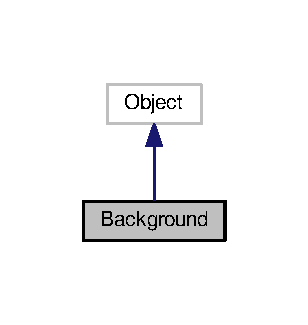
\includegraphics[width=148pt]{classBackground__inherit__graph}
\end{center}
\end{figure}


Collaboration diagram for Background\+:
\nopagebreak
\begin{figure}[H]
\begin{center}
\leavevmode
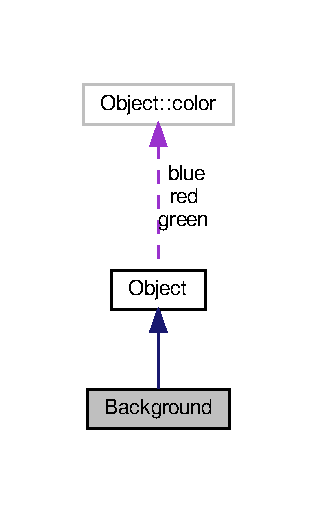
\includegraphics[width=152pt]{classBackground__coll__graph}
\end{center}
\end{figure}
\subsection*{Public Member Functions}
\begin{DoxyCompactItemize}
\item 
void \hyperlink{classBackground_ae0b55ad792ad37c5d7c200c47ff09859}{set\+Background} (string file, int w, int h, S\+D\+L\+\_\+\+Renderer $\ast$ren)\hypertarget{classBackground_ae0b55ad792ad37c5d7c200c47ff09859}{}\label{classBackground_ae0b55ad792ad37c5d7c200c47ff09859}

\begin{DoxyCompactList}\small\item\em Sets the background with a path to the file name, the width and height of the screen, and the renderer. \end{DoxyCompactList}\end{DoxyCompactItemize}
\subsection*{Additional Inherited Members}


\subsection{Detailed Description}
\hyperlink{classObject}{Object} that is a background image that covers the screen. 

Definition at line 7 of file background.\+h.



The documentation for this class was generated from the following files\+:\begin{DoxyCompactItemize}
\item 
background.\+h\item 
background.\+cpp\end{DoxyCompactItemize}

\hypertarget{classCollision}{}\section{Collision Class Reference}
\label{classCollision}\index{Collision@{Collision}}


Class used for calculating different types of collision between given Objects.  




{\ttfamily \#include $<$arch.\+h$>$}

\subsection*{Public Member Functions}
\begin{DoxyCompactItemize}
\item 
bool \hyperlink{classCollision_ae005eb1d857f6127b2673aecacbbd03f}{is\+Touching} (\hyperlink{classObject}{Object} a, \hyperlink{classObject}{Object} b)\hypertarget{classCollision_ae005eb1d857f6127b2673aecacbbd03f}{}\label{classCollision_ae005eb1d857f6127b2673aecacbbd03f}

\begin{DoxyCompactList}\small\item\em Check if two objects are touching. \end{DoxyCompactList}\item 
bool \hyperlink{classCollision_a4fae301767751ae007e953d1d2f49e7b}{out\+Of\+Bounds\+Of} (\hyperlink{classObject}{Object} a, \hyperlink{classObject}{Object} b)\hypertarget{classCollision_a4fae301767751ae007e953d1d2f49e7b}{}\label{classCollision_a4fae301767751ae007e953d1d2f49e7b}

\begin{DoxyCompactList}\small\item\em Check if two object are not touching. \end{DoxyCompactList}\item 
bool \hyperlink{classCollision_aecbf1758ca3a93a39568dbdf87213f20}{is\+Above} (\hyperlink{classObject}{Object} a, \hyperlink{classObject}{Object} b)\hypertarget{classCollision_aecbf1758ca3a93a39568dbdf87213f20}{}\label{classCollision_aecbf1758ca3a93a39568dbdf87213f20}

\begin{DoxyCompactList}\small\item\em Check if the first object is above the second object. \end{DoxyCompactList}\item 
bool \hyperlink{classCollision_ad5414ecc098c7d63155aea827c7d68b1}{is\+Below} (\hyperlink{classObject}{Object} a, \hyperlink{classObject}{Object} b)\hypertarget{classCollision_ad5414ecc098c7d63155aea827c7d68b1}{}\label{classCollision_ad5414ecc098c7d63155aea827c7d68b1}

\begin{DoxyCompactList}\small\item\em Check if the first object is below the second object. \end{DoxyCompactList}\item 
bool \hyperlink{classCollision_a9330290516beca87905e81a974ffca83}{is\+Right\+Of} (\hyperlink{classObject}{Object} a, \hyperlink{classObject}{Object} b)\hypertarget{classCollision_a9330290516beca87905e81a974ffca83}{}\label{classCollision_a9330290516beca87905e81a974ffca83}

\begin{DoxyCompactList}\small\item\em Check if the first object is to the right of the second object. \end{DoxyCompactList}\item 
bool \hyperlink{classCollision_aea67f8b0cd9b37408e2f6f65006b27d3}{is\+Left\+Of} (\hyperlink{classObject}{Object} a, \hyperlink{classObject}{Object} b)\hypertarget{classCollision_aea67f8b0cd9b37408e2f6f65006b27d3}{}\label{classCollision_aea67f8b0cd9b37408e2f6f65006b27d3}

\begin{DoxyCompactList}\small\item\em Check if the first object is to the left of the second object. \end{DoxyCompactList}\item 
bool \hyperlink{classCollision_ae005eb1d857f6127b2673aecacbbd03f}{is\+Touching} (\hyperlink{classObject}{Object} a, \hyperlink{classObject}{Object} b)\hypertarget{classCollision_ae005eb1d857f6127b2673aecacbbd03f}{}\label{classCollision_ae005eb1d857f6127b2673aecacbbd03f}

\begin{DoxyCompactList}\small\item\em Check if two objects are touching. \end{DoxyCompactList}\item 
bool \hyperlink{classCollision_a4fae301767751ae007e953d1d2f49e7b}{out\+Of\+Bounds\+Of} (\hyperlink{classObject}{Object} a, \hyperlink{classObject}{Object} b)\hypertarget{classCollision_a4fae301767751ae007e953d1d2f49e7b}{}\label{classCollision_a4fae301767751ae007e953d1d2f49e7b}

\begin{DoxyCompactList}\small\item\em Check if two object are not touching. \end{DoxyCompactList}\item 
bool \hyperlink{classCollision_aecbf1758ca3a93a39568dbdf87213f20}{is\+Above} (\hyperlink{classObject}{Object} a, \hyperlink{classObject}{Object} b)\hypertarget{classCollision_aecbf1758ca3a93a39568dbdf87213f20}{}\label{classCollision_aecbf1758ca3a93a39568dbdf87213f20}

\begin{DoxyCompactList}\small\item\em Check if the first object is above the second object. \end{DoxyCompactList}\item 
bool \hyperlink{classCollision_ad5414ecc098c7d63155aea827c7d68b1}{is\+Below} (\hyperlink{classObject}{Object} a, \hyperlink{classObject}{Object} b)\hypertarget{classCollision_ad5414ecc098c7d63155aea827c7d68b1}{}\label{classCollision_ad5414ecc098c7d63155aea827c7d68b1}

\begin{DoxyCompactList}\small\item\em Check if the first object is below the second object. \end{DoxyCompactList}\item 
bool \hyperlink{classCollision_a9330290516beca87905e81a974ffca83}{is\+Right\+Of} (\hyperlink{classObject}{Object} a, \hyperlink{classObject}{Object} b)\hypertarget{classCollision_a9330290516beca87905e81a974ffca83}{}\label{classCollision_a9330290516beca87905e81a974ffca83}

\begin{DoxyCompactList}\small\item\em Check if the first object is to the right of the second object. \end{DoxyCompactList}\item 
bool \hyperlink{classCollision_aea67f8b0cd9b37408e2f6f65006b27d3}{is\+Left\+Of} (\hyperlink{classObject}{Object} a, \hyperlink{classObject}{Object} b)\hypertarget{classCollision_aea67f8b0cd9b37408e2f6f65006b27d3}{}\label{classCollision_aea67f8b0cd9b37408e2f6f65006b27d3}

\begin{DoxyCompactList}\small\item\em Check if the first object is to the left of the second object. \end{DoxyCompactList}\end{DoxyCompactItemize}


\subsection{Detailed Description}
Class used for calculating different types of collision between given Objects. 

Definition at line 23 of file arch.\+h.



The documentation for this class was generated from the following files\+:\begin{DoxyCompactItemize}
\item 
arch.\+h\item 
collision.\+h\item 
collision.\+cpp\end{DoxyCompactItemize}

\hypertarget{classEngine}{}\section{Engine Class Reference}
\label{classEngine}\index{Engine@{Engine}}


Class for declaring an engine, which does basic S\+DL commands like creating the window and renderer.  




{\ttfamily \#include $<$engine.\+h$>$}

\subsection*{Classes}
\begin{DoxyCompactItemize}
\item 
struct \hyperlink{structEngine_1_1color}{color}
\end{DoxyCompactItemize}
\subsection*{Public Member Functions}
\begin{DoxyCompactItemize}
\item 
\mbox{\Hypertarget{classEngine_a8ef7030a089ecb30bbfcb9e43094717a}\label{classEngine_a8ef7030a089ecb30bbfcb9e43094717a}} 
\hyperlink{classEngine_a8ef7030a089ecb30bbfcb9e43094717a}{$\sim$\+Engine} ()
\begin{DoxyCompactList}\small\item\em Decontructs renderer and window and then quits S\+DL. \end{DoxyCompactList}\item 
\mbox{\Hypertarget{classEngine_ac2dab34eea67e7a2c006945ee71a9e42}\label{classEngine_ac2dab34eea67e7a2c006945ee71a9e42}} 
void {\bfseries set\+Gravity} (double g)
\item 
\mbox{\Hypertarget{classEngine_a834148373d85dfc947ec3fcb366f25e6}\label{classEngine_a834148373d85dfc947ec3fcb366f25e6}} 
void {\bfseries set\+Frame\+Rate} (int f)
\item 
\mbox{\Hypertarget{classEngine_a54694ab584e0d9fe82d1c25fb86c99e2}\label{classEngine_a54694ab584e0d9fe82d1c25fb86c99e2}} 
double {\bfseries get\+Gravity} () const
\item 
\mbox{\Hypertarget{classEngine_af02c5fcfad817c5c8bc0a3cacfd9d4f8}\label{classEngine_af02c5fcfad817c5c8bc0a3cacfd9d4f8}} 
S\+D\+L\+\_\+\+Renderer $\ast$ \hyperlink{classEngine_af02c5fcfad817c5c8bc0a3cacfd9d4f8}{init} (string s, const int \&w, const int \&h, int flag)
\begin{DoxyCompactList}\small\item\em Create a window with a given name, width, height, and anyother S\+D\+L\+\_\+\+Window flags. \end{DoxyCompactList}\item 
\mbox{\Hypertarget{classEngine_aca16d18226665d75acad41b48a8da989}\label{classEngine_aca16d18226665d75acad41b48a8da989}} 
S\+D\+L\+\_\+\+Renderer $\ast$ \hyperlink{classEngine_aca16d18226665d75acad41b48a8da989}{init} (string s, const int \&w, const int \&h, int flag, int it)
\begin{DoxyCompactList}\small\item\em Create a window with a given name, width, height, S\+D\+L\+\_\+\+Window flags, and specified S\+D\+L\+\_\+\+Init flags. \end{DoxyCompactList}\item 
\mbox{\Hypertarget{classEngine_a4f80e210f2ae48208eed4ad17c309120}\label{classEngine_a4f80e210f2ae48208eed4ad17c309120}} 
S\+D\+L\+\_\+\+Renderer $\ast$ \hyperlink{classEngine_a4f80e210f2ae48208eed4ad17c309120}{init} (string s, const int \&w, const int \&h, int flag, int x, int y)
\begin{DoxyCompactList}\small\item\em Create a window with a given name, width, height, S\+D\+L\+\_\+\+Window flags, and specified x and y coordinate. \end{DoxyCompactList}\item 
\mbox{\Hypertarget{classEngine_aa96fc831b44b6aae0f499360609c574d}\label{classEngine_aa96fc831b44b6aae0f499360609c574d}} 
S\+D\+L\+\_\+\+Renderer $\ast$ \hyperlink{classEngine_aa96fc831b44b6aae0f499360609c574d}{init} (string s, const int \&w, const int \&h, int flag, int x, int y, int it)
\begin{DoxyCompactList}\small\item\em Create a window with a given name, width, height, S\+D\+L\+\_\+\+Window flags, specified x and y coordinate, and S\+D\+L\+\_\+\+Init flags. \end{DoxyCompactList}\item 
\mbox{\Hypertarget{classEngine_ae59bcd31693811574953ba835ecb09bb}\label{classEngine_ae59bcd31693811574953ba835ecb09bb}} 
void \hyperlink{classEngine_ae59bcd31693811574953ba835ecb09bb}{set\+Name} (string s)
\begin{DoxyCompactList}\small\item\em Set window name. \end{DoxyCompactList}\item 
\mbox{\Hypertarget{classEngine_a6133368973d175ef8915cc8033958b2b}\label{classEngine_a6133368973d175ef8915cc8033958b2b}} 
void \hyperlink{classEngine_a6133368973d175ef8915cc8033958b2b}{set\+Pos} (int x, int y)
\begin{DoxyCompactList}\small\item\em Set window position. \end{DoxyCompactList}\item 
\mbox{\Hypertarget{classEngine_ada9e7e5de3b47113fc39fcabfe298f9e}\label{classEngine_ada9e7e5de3b47113fc39fcabfe298f9e}} 
void \hyperlink{classEngine_ada9e7e5de3b47113fc39fcabfe298f9e}{set\+Size} (int w, int y)
\begin{DoxyCompactList}\small\item\em Set window size. \end{DoxyCompactList}\item 
\mbox{\Hypertarget{classEngine_ae42b73be55ab0fa034a0f7dea156cf9c}\label{classEngine_ae42b73be55ab0fa034a0f7dea156cf9c}} 
S\+D\+L\+\_\+\+Renderer $\ast$ \hyperlink{classEngine_ae42b73be55ab0fa034a0f7dea156cf9c}{get\+Renderer} ()
\begin{DoxyCompactList}\small\item\em Returns screen renderer. \end{DoxyCompactList}\item 
\mbox{\Hypertarget{classEngine_ac54bbc31578a1d5fd14887ceaba73843}\label{classEngine_ac54bbc31578a1d5fd14887ceaba73843}} 
S\+D\+L\+\_\+\+Window $\ast$ \hyperlink{classEngine_ac54bbc31578a1d5fd14887ceaba73843}{get\+Window} () const
\begin{DoxyCompactList}\small\item\em Returns screen window. \end{DoxyCompactList}\item 
\mbox{\Hypertarget{classEngine_aeee842a402f260e38e0502e1d95b920b}\label{classEngine_aeee842a402f260e38e0502e1d95b920b}} 
void \hyperlink{classEngine_aeee842a402f260e38e0502e1d95b920b}{set\+Color} (Uint8 r, Uint8 g, Uint8 b)
\begin{DoxyCompactList}\small\item\em Sets S\+DL color. \end{DoxyCompactList}\item 
\mbox{\Hypertarget{classEngine_ad7602820f1b9d75ec1b59f2a6111085e}\label{classEngine_ad7602820f1b9d75ec1b59f2a6111085e}} 
void \hyperlink{classEngine_ad7602820f1b9d75ec1b59f2a6111085e}{loop\+Start} ()
\begin{DoxyCompactList}\small\item\em Call this at the beginning of a loop to initilaize the loop. \end{DoxyCompactList}\item 
\mbox{\Hypertarget{classEngine_a7960743aefd62e846e7f3cd92c18bc73}\label{classEngine_a7960743aefd62e846e7f3cd92c18bc73}} 
void \hyperlink{classEngine_a7960743aefd62e846e7f3cd92c18bc73}{render} ()
\begin{DoxyCompactList}\small\item\em Call this at the end of the game loop to render. \end{DoxyCompactList}\item 
void \hyperlink{classEngine_ad2ff110d5a86c1cd60b541d65915ac48}{update} ()
\begin{DoxyCompactList}\small\item\em Get fps. \end{DoxyCompactList}\item 
\mbox{\Hypertarget{classEngine_a690ac76faed3d2a9f1f582a2e6fc8c85}\label{classEngine_a690ac76faed3d2a9f1f582a2e6fc8c85}} 
void \hyperlink{classEngine_a690ac76faed3d2a9f1f582a2e6fc8c85}{set\+Background} (\hyperlink{classBackground}{Background} b)
\begin{DoxyCompactList}\small\item\em Set background. \end{DoxyCompactList}\item 
\mbox{\Hypertarget{classEngine_a376e4a1ba9adc079e1da9b28a290abd2}\label{classEngine_a376e4a1ba9adc079e1da9b28a290abd2}} 
void \hyperlink{classEngine_a376e4a1ba9adc079e1da9b28a290abd2}{set\+Background} (string filename)
\begin{DoxyCompactList}\small\item\em Set background with filename. \end{DoxyCompactList}\item 
\mbox{\Hypertarget{classEngine_ab55a40463918efa8469cb17c7237e7a7}\label{classEngine_ab55a40463918efa8469cb17c7237e7a7}} 
\hyperlink{classBackground}{Background} \hyperlink{classEngine_ab55a40463918efa8469cb17c7237e7a7}{get\+Background} () const
\begin{DoxyCompactList}\small\item\em Get background. \end{DoxyCompactList}\item 
\mbox{\Hypertarget{classEngine_aa84c13e84d00fd3b0389a9a076ec194f}\label{classEngine_aa84c13e84d00fd3b0389a9a076ec194f}} 
void \hyperlink{classEngine_aa84c13e84d00fd3b0389a9a076ec194f}{draw\+Background} ()
\begin{DoxyCompactList}\small\item\em Draw background. \end{DoxyCompactList}\item 
\mbox{\Hypertarget{classEngine_a276e63ae5648c36051c21c5b7c5dfb4b}\label{classEngine_a276e63ae5648c36051c21c5b7c5dfb4b}} 
void \hyperlink{classEngine_a276e63ae5648c36051c21c5b7c5dfb4b}{draw} (\hyperlink{classObject}{Object} obj)
\begin{DoxyCompactList}\small\item\em Draw an object on the screen. \end{DoxyCompactList}\item 
\mbox{\Hypertarget{classEngine_a212b1b788cae7931fda927c0cbd2e165}\label{classEngine_a212b1b788cae7931fda927c0cbd2e165}} 
void \hyperlink{classEngine_a212b1b788cae7931fda927c0cbd2e165}{draw} (vector$<$ \hyperlink{classObject}{Object} $>$ objs)
\begin{DoxyCompactList}\small\item\em Draw a vector of Objects. \end{DoxyCompactList}\item 
\mbox{\Hypertarget{classEngine_afa41c75e3e6f47f5af9b7ad649d05564}\label{classEngine_afa41c75e3e6f47f5af9b7ad649d05564}} 
void {\bfseries draw} (vector$<$ vector$<$ \hyperlink{classObject}{Object} $>$$>$ objs)
\item 
\mbox{\Hypertarget{classEngine_a81d89df09ee2577fd7deaf2f5e27f93a}\label{classEngine_a81d89df09ee2577fd7deaf2f5e27f93a}} 
void \hyperlink{classEngine_a81d89df09ee2577fd7deaf2f5e27f93a}{draw} (\hyperlink{classObject}{Object} obj, int key)
\begin{DoxyCompactList}\small\item\em Draw an object with a pass key before/during splash. \end{DoxyCompactList}\item 
\mbox{\Hypertarget{classEngine_a9435c9399f0d3952032c106e7ee8f6e9}\label{classEngine_a9435c9399f0d3952032c106e7ee8f6e9}} 
void \hyperlink{classEngine_a9435c9399f0d3952032c106e7ee8f6e9}{draw} (\hyperlink{classLevel}{Level} lvl)
\begin{DoxyCompactList}\small\item\em Draw the level. \end{DoxyCompactList}\item 
\mbox{\Hypertarget{classEngine_acfa5f40b14195633d084fdb54deffcc9}\label{classEngine_acfa5f40b14195633d084fdb54deffcc9}} 
void \hyperlink{classEngine_acfa5f40b14195633d084fdb54deffcc9}{draw} (const char $\ast$text, int x, int y, int r, int g, int b)
\begin{DoxyCompactList}\small\item\em Write to the screen with a char, coordinates, color, ttf file. \end{DoxyCompactList}\item 
\mbox{\Hypertarget{classEngine_adb6f1426c5c57f9d60be1e10d8eb2506}\label{classEngine_adb6f1426c5c57f9d60be1e10d8eb2506}} 
void \hyperlink{classEngine_adb6f1426c5c57f9d60be1e10d8eb2506}{splash} ()
\begin{DoxyCompactList}\small\item\em Calls splashscreen at the beginning of the game. This is automatically called unless deactivated. \end{DoxyCompactList}\item 
\mbox{\Hypertarget{classEngine_a3b9cf8a050f43e4e185748f7b2a3ded8}\label{classEngine_a3b9cf8a050f43e4e185748f7b2a3ded8}} 
void \hyperlink{classEngine_a3b9cf8a050f43e4e185748f7b2a3ded8}{bypass\+Splash} (int key)
\begin{DoxyCompactList}\small\item\em Deactives the splashscreen, requires key. \end{DoxyCompactList}\item 
\mbox{\Hypertarget{classEngine_aabab82c2ba4dca772a28dbbd4fe08cb4}\label{classEngine_aabab82c2ba4dca772a28dbbd4fe08cb4}} 
bool \hyperlink{classEngine_aabab82c2ba4dca772a28dbbd4fe08cb4}{has\+Splashed} ()
\begin{DoxyCompactList}\small\item\em Check if the splashscreen has occured. \end{DoxyCompactList}\item 
\mbox{\Hypertarget{classEngine_a60d5307c4bc5005119086ff9f3e21624}\label{classEngine_a60d5307c4bc5005119086ff9f3e21624}} 
void \hyperlink{classEngine_a60d5307c4bc5005119086ff9f3e21624}{debug\+Mode} (bool d)
\begin{DoxyCompactList}\small\item\em Active debugger with Boolean. \end{DoxyCompactList}\item 
\mbox{\Hypertarget{classEngine_a4be41373ed9a4b0d14f256ce777a2c3d}\label{classEngine_a4be41373ed9a4b0d14f256ce777a2c3d}} 
void {\bfseries load\+Font} (char $\ast$font\+\_\+path)
\item 
\mbox{\Hypertarget{classEngine_a4b1936a48e82bbb7af8b3be97f2e2816}\label{classEngine_a4b1936a48e82bbb7af8b3be97f2e2816}} 
void \hyperlink{classEngine_a4b1936a48e82bbb7af8b3be97f2e2816}{set\+Font\+Color} (int r, int g, int b)
\begin{DoxyCompactList}\small\item\em Set Font Color Using R\+GB. \end{DoxyCompactList}\item 
\mbox{\Hypertarget{classEngine_ab28645d6809f5335cc9034caaba38827}\label{classEngine_ab28645d6809f5335cc9034caaba38827}} 
void {\bfseries hide\+Mouse} ()
\item 
\mbox{\Hypertarget{classEngine_a6d476e93e46e59543ea9714b93a30936}\label{classEngine_a6d476e93e46e59543ea9714b93a30936}} 
void {\bfseries show\+Mouse} ()
\item 
\mbox{\Hypertarget{classEngine_a21347f05ca9d124cbb22fb73545de858}\label{classEngine_a21347f05ca9d124cbb22fb73545de858}} 
bool {\bfseries get\+Running} () const
\item 
\mbox{\Hypertarget{classEngine_ac5a84be825afebf377e227bcb049a753}\label{classEngine_ac5a84be825afebf377e227bcb049a753}} 
void {\bfseries set\+Running} (bool r)
\item 
\mbox{\Hypertarget{classEngine_ad5387289f39246870a3c40d61b31fed8}\label{classEngine_ad5387289f39246870a3c40d61b31fed8}} 
void {\bfseries set\+G\+L\+View} (int a, int b, int c, int d, int e, int f, int g, int h, int i)
\item 
\mbox{\Hypertarget{classEngine_a0ac77a2abc0269f3825a184fbfcef3dd}\label{classEngine_a0ac77a2abc0269f3825a184fbfcef3dd}} 
void {\bfseries set\+G\+L\+Mode} (bool m)
\item 
\mbox{\Hypertarget{classEngine_a030675a3b74445ea6c19073594510fdf}\label{classEngine_a030675a3b74445ea6c19073594510fdf}} 
int {\bfseries get\+F\+PS} () const
\item 
\mbox{\Hypertarget{classEngine_a514f8d788ced7c6508b8b6f9ef66ccb1}\label{classEngine_a514f8d788ced7c6508b8b6f9ef66ccb1}} 
void {\bfseries loop} ()
\item 
\mbox{\Hypertarget{classEngine_adfac6631b6c52bcb43811742aa172d9d}\label{classEngine_adfac6631b6c52bcb43811742aa172d9d}} 
int {\bfseries get\+Ticks} ()
\item 
\mbox{\Hypertarget{classEngine_a15aa4850592df8924eb542ff0709bd98}\label{classEngine_a15aa4850592df8924eb542ff0709bd98}} 
void {\bfseries delay} (int time)
\item 
\mbox{\Hypertarget{classEngine_a74e701ab9fb6a69713f9867d9962630e}\label{classEngine_a74e701ab9fb6a69713f9867d9962630e}} 
void {\bfseries enable\+Transparency} ()
\item 
\mbox{\Hypertarget{classEngine_ab0353877b7da9431718029c77db2d35d}\label{classEngine_ab0353877b7da9431718029c77db2d35d}} 
void {\bfseries set\+Gamestate} (int s)
\item 
\mbox{\Hypertarget{classEngine_aba0938d28018a9ed9bcea2a78c28b972}\label{classEngine_aba0938d28018a9ed9bcea2a78c28b972}} 
int {\bfseries get\+Game\+State} ()
\item 
\mbox{\Hypertarget{classEngine_a095fb17299a5a7eac3acd98dceff6fd3}\label{classEngine_a095fb17299a5a7eac3acd98dceff6fd3}} 
void {\bfseries set\+Splash\+Color} (int r, int g, int b)
\end{DoxyCompactItemize}


\subsection{Detailed Description}
Class for declaring an engine, which does basic S\+DL commands like creating the window and renderer. 

Definition at line 36 of file engine.\+h.



\subsection{Member Function Documentation}
\mbox{\Hypertarget{classEngine_ad2ff110d5a86c1cd60b541d65915ac48}\label{classEngine_ad2ff110d5a86c1cd60b541d65915ac48}} 
\index{Engine@{Engine}!update@{update}}
\index{update@{update}!Engine@{Engine}}
\subsubsection{\texorpdfstring{update()}{update()}}
{\footnotesize\ttfamily void Engine\+::update (\begin{DoxyParamCaption}{ }\end{DoxyParamCaption})}



Get fps. 

Update loop time. 

Definition at line 135 of file engine.\+cpp.


\begin{DoxyCode}
135                     \{
136   \textcolor{comment}{//simulationTime += 16;}
137   \textcolor{comment}{//if(simulationTime < realTime) \{ fps = true; \} else \{ fps = false; \}}
138   \textcolor{keywordflow}{if}(glMode) \{
139    glClear( GL\_COLOR\_BUFFER\_BIT | GL\_DEPTH\_BUFFER\_BIT);
140    glMatrixMode( GL\_MODELVIEW );
141    glLoadIdentity( );
142    gluLookAt(glView[0],glView[1],glView[2],glView[3],glView[4],glView[5],glView[6],glView[7],glView[8]);
143   \}
144 \}
\end{DoxyCode}


The documentation for this class was generated from the following files\+:\begin{DoxyCompactItemize}
\item 
engine.\+h\item 
engine.\+cpp\end{DoxyCompactItemize}

\hypertarget{classEntity}{}\section{Entity Class Reference}
\label{classEntity}\index{Entity@{Entity}}


Class for storing health, emotion, team, etc. of an \hyperlink{classObject}{Object}.  




{\ttfamily \#include $<$entity.\+h$>$}



Inheritance diagram for Entity\+:\nopagebreak
\begin{figure}[H]
\begin{center}
\leavevmode
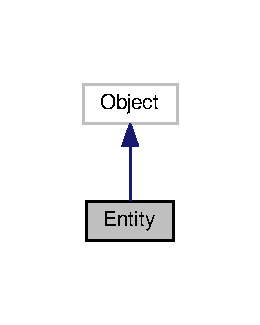
\includegraphics[width=125pt]{classEntity__inherit__graph}
\end{center}
\end{figure}


Collaboration diagram for Entity\+:\nopagebreak
\begin{figure}[H]
\begin{center}
\leavevmode
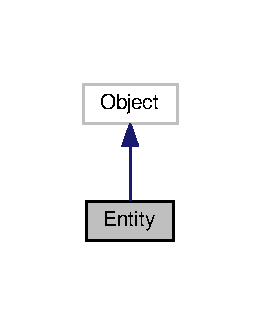
\includegraphics[width=152pt]{classEntity__coll__graph}
\end{center}
\end{figure}
\subsection*{Public Member Functions}
\begin{DoxyCompactItemize}
\item 
\mbox{\Hypertarget{classEntity_a7d65c1c4303715382272f6065e29ac03}\label{classEntity_a7d65c1c4303715382272f6065e29ac03}} 
double \hyperlink{classEntity_a7d65c1c4303715382272f6065e29ac03}{get\+Health} () const
\begin{DoxyCompactList}\small\item\em Get \hyperlink{classEntity}{Entity}\textquotesingle{}s health. \end{DoxyCompactList}\item 
\mbox{\Hypertarget{classEntity_a4f521d321ea874c474cc0506ff78da08}\label{classEntity_a4f521d321ea874c474cc0506ff78da08}} 
void \hyperlink{classEntity_a4f521d321ea874c474cc0506ff78da08}{set\+Health} (double h)
\begin{DoxyCompactList}\small\item\em Set the \hyperlink{classEntity}{Entity}\textquotesingle{}s health. If the health is higher then the max health it will set it to the max health. \end{DoxyCompactList}\item 
\mbox{\Hypertarget{classEntity_ad1e0ca19eb67af423f6803b52b351618}\label{classEntity_ad1e0ca19eb67af423f6803b52b351618}} 
double \hyperlink{classEntity_ad1e0ca19eb67af423f6803b52b351618}{get\+Max\+Health} () const
\begin{DoxyCompactList}\small\item\em Get max health. \end{DoxyCompactList}\item 
\mbox{\Hypertarget{classEntity_a375385b808ac7fd4632d6b71f15b0e1c}\label{classEntity_a375385b808ac7fd4632d6b71f15b0e1c}} 
void \hyperlink{classEntity_a375385b808ac7fd4632d6b71f15b0e1c}{set\+Max\+Health} (double mh)
\begin{DoxyCompactList}\small\item\em Set max health. \end{DoxyCompactList}\item 
\mbox{\Hypertarget{classEntity_af7fb432e778f9fcfe4584d09b6a73294}\label{classEntity_af7fb432e778f9fcfe4584d09b6a73294}} 
void \hyperlink{classEntity_af7fb432e778f9fcfe4584d09b6a73294}{damage} (double d)
\begin{DoxyCompactList}\small\item\em Deal damage. Subtracted from health. If health is less then zero it kills the entity. \end{DoxyCompactList}\item 
\mbox{\Hypertarget{classEntity_aef00fa78f66829c0ecb8c27c65bd3a92}\label{classEntity_aef00fa78f66829c0ecb8c27c65bd3a92}} 
void \hyperlink{classEntity_aef00fa78f66829c0ecb8c27c65bd3a92}{heal} (double h)
\begin{DoxyCompactList}\small\item\em Give health to the \hyperlink{classEntity}{Entity}. \end{DoxyCompactList}\item 
\mbox{\Hypertarget{classEntity_a515356280cfc50f988c01d800bc8947e}\label{classEntity_a515356280cfc50f988c01d800bc8947e}} 
int \hyperlink{classEntity_a515356280cfc50f988c01d800bc8947e}{get\+Emotion} () const
\begin{DoxyCompactList}\small\item\em Get current emotion state. \end{DoxyCompactList}\item 
\mbox{\Hypertarget{classEntity_a79056ef5d580c09fe6cf34b989b14589}\label{classEntity_a79056ef5d580c09fe6cf34b989b14589}} 
void \hyperlink{classEntity_a79056ef5d580c09fe6cf34b989b14589}{set\+Emotion} (int e)
\begin{DoxyCompactList}\small\item\em Set current emotion state. \end{DoxyCompactList}\item 
\mbox{\Hypertarget{classEntity_a3d1b7fa592ea11e57323212e88d67830}\label{classEntity_a3d1b7fa592ea11e57323212e88d67830}} 
int \hyperlink{classEntity_a3d1b7fa592ea11e57323212e88d67830}{get\+Team} () const
\begin{DoxyCompactList}\small\item\em Get \hyperlink{classEntity}{Entity}\textquotesingle{}s team. \end{DoxyCompactList}\item 
\mbox{\Hypertarget{classEntity_a9fe88f82909f89087ad17d4d7ce6b22e}\label{classEntity_a9fe88f82909f89087ad17d4d7ce6b22e}} 
void \hyperlink{classEntity_a9fe88f82909f89087ad17d4d7ce6b22e}{set\+Team} (int t)
\begin{DoxyCompactList}\small\item\em Set \hyperlink{classEntity}{Entity}\textquotesingle{}s team. \end{DoxyCompactList}\item 
\mbox{\Hypertarget{classEntity_aea1c1568b4123d989c5310697030ad77}\label{classEntity_aea1c1568b4123d989c5310697030ad77}} 
bool \hyperlink{classEntity_aea1c1568b4123d989c5310697030ad77}{is\+Active} () const
\begin{DoxyCompactList}\small\item\em Check if \hyperlink{classEntity}{Entity} is active. \end{DoxyCompactList}\item 
\mbox{\Hypertarget{classEntity_a522648b330daab91b49f78f0737a943f}\label{classEntity_a522648b330daab91b49f78f0737a943f}} 
void \hyperlink{classEntity_a522648b330daab91b49f78f0737a943f}{kill} ()
\begin{DoxyCompactList}\small\item\em Sets health to zero and deactives the \hyperlink{classEntity}{Entity}. \end{DoxyCompactList}\item 
\mbox{\Hypertarget{classEntity_aa409e70e0f5abb2ac1314f8745b9a661}\label{classEntity_aa409e70e0f5abb2ac1314f8745b9a661}} 
void \hyperlink{classEntity_aa409e70e0f5abb2ac1314f8745b9a661}{deactivate} ()
\begin{DoxyCompactList}\small\item\em Sets active to false. \end{DoxyCompactList}\item 
\mbox{\Hypertarget{classEntity_a95079be1c9fa9f109dd3cf7446eeeb1d}\label{classEntity_a95079be1c9fa9f109dd3cf7446eeeb1d}} 
void \hyperlink{classEntity_a95079be1c9fa9f109dd3cf7446eeeb1d}{activate} ()
\begin{DoxyCompactList}\small\item\em Sets active to true. \end{DoxyCompactList}\item 
\mbox{\Hypertarget{classEntity_a63aac9638f79f0608b08f28b8cdc718e}\label{classEntity_a63aac9638f79f0608b08f28b8cdc718e}} 
void \hyperlink{classEntity_a63aac9638f79f0608b08f28b8cdc718e}{check\+Displayable} (\hyperlink{classObject}{Object} screen)
\begin{DoxyCompactList}\small\item\em Checks if an the \hyperlink{classEntity}{Entity} is in the current screen by passing the screen to it. \end{DoxyCompactList}\item 
\mbox{\Hypertarget{classEntity_a2ea4a13ae5345fb4bb0ccc299011e209}\label{classEntity_a2ea4a13ae5345fb4bb0ccc299011e209}} 
S\+D\+L\+\_\+\+Rect \hyperlink{classEntity_a2ea4a13ae5345fb4bb0ccc299011e209}{get\+Detect} () const
\begin{DoxyCompactList}\small\item\em Returns the detection radius. \end{DoxyCompactList}\item 
\mbox{\Hypertarget{classEntity_a7624a9b21bbb1bd97d7f2eac20339a82}\label{classEntity_a7624a9b21bbb1bd97d7f2eac20339a82}} 
void \hyperlink{classEntity_a7624a9b21bbb1bd97d7f2eac20339a82}{set\+Detect} (S\+D\+L\+\_\+\+Rect d)
\begin{DoxyCompactList}\small\item\em Sets the detection with another S\+D\+L\+\_\+\+Rect. \end{DoxyCompactList}\item 
\mbox{\Hypertarget{classEntity_a884a7f8a537f3d0e926dfedb8e88a740}\label{classEntity_a884a7f8a537f3d0e926dfedb8e88a740}} 
void \hyperlink{classEntity_a884a7f8a537f3d0e926dfedb8e88a740}{set\+Detect\+Range} (int r)
\begin{DoxyCompactList}\small\item\em Sets the detection radius with a single given distance. \end{DoxyCompactList}\item 
\mbox{\Hypertarget{classEntity_af4b91451301036e4aed029e90a7ba726}\label{classEntity_af4b91451301036e4aed029e90a7ba726}} 
void \hyperlink{classEntity_af4b91451301036e4aed029e90a7ba726}{set\+Detect\+Range} (int w, int h)
\begin{DoxyCompactList}\small\item\em Sets the detection radius with two given distances in both directions. \end{DoxyCompactList}\end{DoxyCompactItemize}
\subsection*{Additional Inherited Members}


\subsection{Detailed Description}
Class for storing health, emotion, team, etc. of an \hyperlink{classObject}{Object}. 

Definition at line 9 of file entity.\+h.



The documentation for this class was generated from the following files\+:\begin{DoxyCompactItemize}
\item 
entity.\+h\item 
entity.\+cpp\end{DoxyCompactItemize}

\hypertarget{classGameState}{}\section{Game\+State Class Reference}
\label{classGameState}\index{Game\+State@{Game\+State}}
\subsection*{Public Member Functions}
\begin{DoxyCompactItemize}
\item 
int {\bfseries get\+Game\+State} ()\hypertarget{classGameState_af20f310030244f07204b2e53b364332e}{}\label{classGameState_af20f310030244f07204b2e53b364332e}

\item 
void {\bfseries set\+Game\+State} (int)\hypertarget{classGameState_abb0ab40349a3094465a74643eb731e22}{}\label{classGameState_abb0ab40349a3094465a74643eb731e22}

\item 
int {\bfseries get\+Game\+State} ()\hypertarget{classGameState_af20f310030244f07204b2e53b364332e}{}\label{classGameState_af20f310030244f07204b2e53b364332e}

\item 
void {\bfseries set\+Game\+State} (int)\hypertarget{classGameState_abb0ab40349a3094465a74643eb731e22}{}\label{classGameState_abb0ab40349a3094465a74643eb731e22}

\end{DoxyCompactItemize}
\subsection*{Public Attributes}
\begin{DoxyCompactItemize}
\item 
int {\bfseries S\+P\+L\+A\+SH} = 0\hypertarget{classGameState_ade9e04b33f1dea1d62358a4f63b9a509}{}\label{classGameState_ade9e04b33f1dea1d62358a4f63b9a509}

\item 
int {\bfseries M\+E\+NU} = 1\hypertarget{classGameState_abd9f3d7cdc22931db952cc17010752a1}{}\label{classGameState_abd9f3d7cdc22931db952cc17010752a1}

\item 
int {\bfseries I\+N\+G\+A\+ME} = 2\hypertarget{classGameState_aae6641ae96366549f729c136cdcc5c5c}{}\label{classGameState_aae6641ae96366549f729c136cdcc5c5c}

\item 
int {\bfseries G\+A\+M\+E\+O\+V\+ER} = 3\hypertarget{classGameState_a994c426ab97d2c6e186c13fd357ccc68}{}\label{classGameState_a994c426ab97d2c6e186c13fd357ccc68}

\item 
int {\bfseries P\+A\+U\+SE} = 4\hypertarget{classGameState_a1353d084bf0c63bd879656de599db4b5}{}\label{classGameState_a1353d084bf0c63bd879656de599db4b5}

\end{DoxyCompactItemize}


\subsection{Detailed Description}


Definition at line 214 of file arch.\+h.



The documentation for this class was generated from the following files\+:\begin{DoxyCompactItemize}
\item 
arch.\+h\item 
gamestate.\+h\item 
gamestate.\+cpp\end{DoxyCompactItemize}

\hypertarget{classImage}{}\section{Image Class Reference}
\label{classImage}\index{Image@{Image}}


Class for loading in S\+DL Textures.  




{\ttfamily \#include $<$arch.\+h$>$}

\subsection*{Public Member Functions}
\begin{DoxyCompactItemize}
\item 
void \hyperlink{classImage_a776ab55f3884f994512aa092cd7fa250}{load\+Image} (string file, S\+D\+L\+\_\+\+Renderer $\ast$ren)\hypertarget{classImage_a776ab55f3884f994512aa092cd7fa250}{}\label{classImage_a776ab55f3884f994512aa092cd7fa250}

\begin{DoxyCompactList}\small\item\em Load in either a B\+MP or P\+NG file with the path and renderer. \end{DoxyCompactList}\item 
void \hyperlink{classImage_ab00c4a53e3154287075c956c805e1cb1}{load\+P\+NG} (string file, S\+D\+L\+\_\+\+Renderer $\ast$ren)\hypertarget{classImage_ab00c4a53e3154287075c956c805e1cb1}{}\label{classImage_ab00c4a53e3154287075c956c805e1cb1}

\begin{DoxyCompactList}\small\item\em Load in a P\+NG image with the path to the P\+NG file and the renderer. \end{DoxyCompactList}\item 
void \hyperlink{classImage_ad37ad8bd7d9572be7fbbd921a299d235}{load\+B\+MP} (string file, S\+D\+L\+\_\+\+Renderer $\ast$ren)\hypertarget{classImage_ad37ad8bd7d9572be7fbbd921a299d235}{}\label{classImage_ad37ad8bd7d9572be7fbbd921a299d235}

\begin{DoxyCompactList}\small\item\em Load in a B\+MP image with the path to the B\+MP file and the renderer. \end{DoxyCompactList}\item 
S\+D\+L\+\_\+\+Texture $\ast$ \hyperlink{classImage_a6312e473b9315c6db49fbd284b5cf81a}{get\+Texture} ()\hypertarget{classImage_a6312e473b9315c6db49fbd284b5cf81a}{}\label{classImage_a6312e473b9315c6db49fbd284b5cf81a}

\begin{DoxyCompactList}\small\item\em Get S\+D\+L\+\_\+\+Texture. \end{DoxyCompactList}\item 
void \hyperlink{classImage_af42b5d6a8abd90d67e9ae19e374520da}{set\+Image} (S\+D\+L\+\_\+\+Texture $\ast$t)\hypertarget{classImage_af42b5d6a8abd90d67e9ae19e374520da}{}\label{classImage_af42b5d6a8abd90d67e9ae19e374520da}

\begin{DoxyCompactList}\small\item\em Set new, preloaded texture, to \hyperlink{classImage}{Image}. \end{DoxyCompactList}\item 
string \hyperlink{classImage_aebc4cdd98961289324e6159b77ee3e69}{get\+File} () const \hypertarget{classImage_aebc4cdd98961289324e6159b77ee3e69}{}\label{classImage_aebc4cdd98961289324e6159b77ee3e69}

\begin{DoxyCompactList}\small\item\em Get path file of the image. \end{DoxyCompactList}\item 
void \hyperlink{classImage_ab4030489c65a25b2e0c458acac0ca94e}{set\+File} (string f)\hypertarget{classImage_ab4030489c65a25b2e0c458acac0ca94e}{}\label{classImage_ab4030489c65a25b2e0c458acac0ca94e}

\begin{DoxyCompactList}\small\item\em Set path file to the image. \end{DoxyCompactList}\item 
void \hyperlink{classImage_a776ab55f3884f994512aa092cd7fa250}{load\+Image} (string file, S\+D\+L\+\_\+\+Renderer $\ast$ren)\hypertarget{classImage_a776ab55f3884f994512aa092cd7fa250}{}\label{classImage_a776ab55f3884f994512aa092cd7fa250}

\begin{DoxyCompactList}\small\item\em Load in either a B\+MP or P\+NG file with the path and renderer. \end{DoxyCompactList}\item 
void \hyperlink{classImage_ab00c4a53e3154287075c956c805e1cb1}{load\+P\+NG} (string file, S\+D\+L\+\_\+\+Renderer $\ast$ren)\hypertarget{classImage_ab00c4a53e3154287075c956c805e1cb1}{}\label{classImage_ab00c4a53e3154287075c956c805e1cb1}

\begin{DoxyCompactList}\small\item\em Load in a P\+NG image with the path to the P\+NG file and the renderer. \end{DoxyCompactList}\item 
void \hyperlink{classImage_ad37ad8bd7d9572be7fbbd921a299d235}{load\+B\+MP} (string file, S\+D\+L\+\_\+\+Renderer $\ast$ren)\hypertarget{classImage_ad37ad8bd7d9572be7fbbd921a299d235}{}\label{classImage_ad37ad8bd7d9572be7fbbd921a299d235}

\begin{DoxyCompactList}\small\item\em Load in a B\+MP image with the path to the B\+MP file and the renderer. \end{DoxyCompactList}\item 
S\+D\+L\+\_\+\+Texture $\ast$ \hyperlink{classImage_a2425ac0fd54cc559ead30cac5b18c29e}{get\+Texture} ()\hypertarget{classImage_a2425ac0fd54cc559ead30cac5b18c29e}{}\label{classImage_a2425ac0fd54cc559ead30cac5b18c29e}

\begin{DoxyCompactList}\small\item\em Get S\+D\+L\+\_\+\+Texture. \end{DoxyCompactList}\item 
void \hyperlink{classImage_af42b5d6a8abd90d67e9ae19e374520da}{set\+Image} (S\+D\+L\+\_\+\+Texture $\ast$t)\hypertarget{classImage_af42b5d6a8abd90d67e9ae19e374520da}{}\label{classImage_af42b5d6a8abd90d67e9ae19e374520da}

\begin{DoxyCompactList}\small\item\em Set new, preloaded texture, to \hyperlink{classImage}{Image}. \end{DoxyCompactList}\item 
string \hyperlink{classImage_aebc4cdd98961289324e6159b77ee3e69}{get\+File} () const \hypertarget{classImage_aebc4cdd98961289324e6159b77ee3e69}{}\label{classImage_aebc4cdd98961289324e6159b77ee3e69}

\begin{DoxyCompactList}\small\item\em Get path file of the image. \end{DoxyCompactList}\item 
void \hyperlink{classImage_ab4030489c65a25b2e0c458acac0ca94e}{set\+File} (string f)\hypertarget{classImage_ab4030489c65a25b2e0c458acac0ca94e}{}\label{classImage_ab4030489c65a25b2e0c458acac0ca94e}

\begin{DoxyCompactList}\small\item\em Set path file to the image. \end{DoxyCompactList}\end{DoxyCompactItemize}


\subsection{Detailed Description}
Class for loading in S\+DL Textures. 

Definition at line 236 of file arch.\+h.



The documentation for this class was generated from the following files\+:\begin{DoxyCompactItemize}
\item 
arch.\+h\item 
image.\+h\item 
image.\+cpp\end{DoxyCompactItemize}

\hypertarget{classInput}{}\section{Input Class Reference}
\label{classInput}\index{Input@{Input}}


Class for checking and storing keyboard and mouse input.  




{\ttfamily \#include $<$input.\+h$>$}

\subsection*{Public Member Functions}
\begin{DoxyCompactItemize}
\item 
void \hyperlink{classInput_a7664a52377e4bda7524d288df481954b}{log\+Press} ()\hypertarget{classInput_a7664a52377e4bda7524d288df481954b}{}\label{classInput_a7664a52377e4bda7524d288df481954b}

\begin{DoxyCompactList}\small\item\em Log all current keys and buttons being pressed. \end{DoxyCompactList}\item 
bool \hyperlink{classInput_a2f5d21366e04e3ce200fe73c6c748dd8}{check\+Key} (int \hyperlink{classInput_aa069678fdc7c45c405c044ed8e45a379}{k})\hypertarget{classInput_a2f5d21366e04e3ce200fe73c6c748dd8}{}\label{classInput_a2f5d21366e04e3ce200fe73c6c748dd8}

\begin{DoxyCompactList}\small\item\em Check if a key has been pressed using a given key from this class. Ex\+: \hyperlink{classInput}{Input} i; i.\+check\+Key(i.\+up);. \end{DoxyCompactList}\item 
void \hyperlink{classInput_a8bec96dd53baf5ec754c199af3c957c8}{reset} ()\hypertarget{classInput_a8bec96dd53baf5ec754c199af3c957c8}{}\label{classInput_a8bec96dd53baf5ec754c199af3c957c8}

\begin{DoxyCompactList}\small\item\em Reset all pressed keystrokes and other inputs to false. Automatically down at the beginning of each \hyperlink{classInput_a7664a52377e4bda7524d288df481954b}{log\+Press()}. \end{DoxyCompactList}\end{DoxyCompactItemize}
\subsection*{Public Attributes}
\begin{DoxyCompactItemize}
\item 
int \hyperlink{classInput_aa5becba821fbe9c146c332091ebcc6f2}{left}\hypertarget{classInput_aa5becba821fbe9c146c332091ebcc6f2}{}\label{classInput_aa5becba821fbe9c146c332091ebcc6f2}

\begin{DoxyCompactList}\small\item\em Log ID for left. \end{DoxyCompactList}\item 
int \hyperlink{classInput_a481ae9265fafe80dad6850a24980bfb5}{right}\hypertarget{classInput_a481ae9265fafe80dad6850a24980bfb5}{}\label{classInput_a481ae9265fafe80dad6850a24980bfb5}

\begin{DoxyCompactList}\small\item\em Log ID for right. \end{DoxyCompactList}\item 
int \hyperlink{classInput_ad83fb715e39bdc509caf1c2bb7bf692d}{up}\hypertarget{classInput_ad83fb715e39bdc509caf1c2bb7bf692d}{}\label{classInput_ad83fb715e39bdc509caf1c2bb7bf692d}

\begin{DoxyCompactList}\small\item\em Log ID for up. \end{DoxyCompactList}\item 
int \hyperlink{classInput_a24c4a5d08fb4de9300931efb8e7787fb}{down}\hypertarget{classInput_a24c4a5d08fb4de9300931efb8e7787fb}{}\label{classInput_a24c4a5d08fb4de9300931efb8e7787fb}

\begin{DoxyCompactList}\small\item\em Log ID for down. \end{DoxyCompactList}\item 
int \hyperlink{classInput_ad1b648983bba177348f968e05dccfb4a}{q}\hypertarget{classInput_ad1b648983bba177348f968e05dccfb4a}{}\label{classInput_ad1b648983bba177348f968e05dccfb4a}

\begin{DoxyCompactList}\small\item\em Log ID for q. \end{DoxyCompactList}\item 
int \hyperlink{classInput_a50cd82a148ff2ee1bd6f1692277ae5d2}{w}\hypertarget{classInput_a50cd82a148ff2ee1bd6f1692277ae5d2}{}\label{classInput_a50cd82a148ff2ee1bd6f1692277ae5d2}

\begin{DoxyCompactList}\small\item\em Log ID for w. \end{DoxyCompactList}\item 
int \hyperlink{classInput_a205664bff534e2f83a63ee2b064eade5}{e}\hypertarget{classInput_a205664bff534e2f83a63ee2b064eade5}{}\label{classInput_a205664bff534e2f83a63ee2b064eade5}

\begin{DoxyCompactList}\small\item\em Log ID for e. \end{DoxyCompactList}\item 
int \hyperlink{classInput_a17daf5dfbf35ddbbab9b51639eef1483}{r}\hypertarget{classInput_a17daf5dfbf35ddbbab9b51639eef1483}{}\label{classInput_a17daf5dfbf35ddbbab9b51639eef1483}

\begin{DoxyCompactList}\small\item\em Log ID for r. \end{DoxyCompactList}\item 
int \hyperlink{classInput_a48796fc892e530c1a07bd53c7450b152}{t}\hypertarget{classInput_a48796fc892e530c1a07bd53c7450b152}{}\label{classInput_a48796fc892e530c1a07bd53c7450b152}

\begin{DoxyCompactList}\small\item\em Log ID for t. \end{DoxyCompactList}\item 
int \hyperlink{classInput_a4311bc1bf1342c70c9d1afdec7735ae1}{y}\hypertarget{classInput_a4311bc1bf1342c70c9d1afdec7735ae1}{}\label{classInput_a4311bc1bf1342c70c9d1afdec7735ae1}

\begin{DoxyCompactList}\small\item\em Log ID for y. \end{DoxyCompactList}\item 
int \hyperlink{classInput_ac67e86cfe0b0fba4fbc9bb894d8b4bc6}{u}\hypertarget{classInput_ac67e86cfe0b0fba4fbc9bb894d8b4bc6}{}\label{classInput_ac67e86cfe0b0fba4fbc9bb894d8b4bc6}

\begin{DoxyCompactList}\small\item\em Log ID for u. \end{DoxyCompactList}\item 
int \hyperlink{classInput_a660fba8643afb44475ad16745e241311}{i}\hypertarget{classInput_a660fba8643afb44475ad16745e241311}{}\label{classInput_a660fba8643afb44475ad16745e241311}

\begin{DoxyCompactList}\small\item\em Log ID for i. \end{DoxyCompactList}\item 
int \hyperlink{classInput_a7bb0c19997b45f748e6014357c70c7cb}{o}\hypertarget{classInput_a7bb0c19997b45f748e6014357c70c7cb}{}\label{classInput_a7bb0c19997b45f748e6014357c70c7cb}

\begin{DoxyCompactList}\small\item\em Log ID for o. \end{DoxyCompactList}\item 
int \hyperlink{classInput_abd6df3e98127cbfeccea2d15b8d1114b}{p}\hypertarget{classInput_abd6df3e98127cbfeccea2d15b8d1114b}{}\label{classInput_abd6df3e98127cbfeccea2d15b8d1114b}

\begin{DoxyCompactList}\small\item\em Log ID for p. \end{DoxyCompactList}\item 
int \hyperlink{classInput_a764eee99000b65d049ca62748cb1d3ea}{a}\hypertarget{classInput_a764eee99000b65d049ca62748cb1d3ea}{}\label{classInput_a764eee99000b65d049ca62748cb1d3ea}

\begin{DoxyCompactList}\small\item\em Log ID for a. \end{DoxyCompactList}\item 
int \hyperlink{classInput_a190adb31d17011c9bc548e35c5165016}{s}\hypertarget{classInput_a190adb31d17011c9bc548e35c5165016}{}\label{classInput_a190adb31d17011c9bc548e35c5165016}

\begin{DoxyCompactList}\small\item\em Log ID for s. \end{DoxyCompactList}\item 
int \hyperlink{classInput_adb7493830556c3f91c9ab6c9c71176cb}{d}\hypertarget{classInput_adb7493830556c3f91c9ab6c9c71176cb}{}\label{classInput_adb7493830556c3f91c9ab6c9c71176cb}

\begin{DoxyCompactList}\small\item\em Log ID for d. \end{DoxyCompactList}\item 
int \hyperlink{classInput_a784801d5726179bf9b6f3d3ec6a800a3}{f}\hypertarget{classInput_a784801d5726179bf9b6f3d3ec6a800a3}{}\label{classInput_a784801d5726179bf9b6f3d3ec6a800a3}

\begin{DoxyCompactList}\small\item\em Log ID for f. \end{DoxyCompactList}\item 
int \hyperlink{classInput_a9646f2b1930e3f67a99d3e642a63e4ac}{g}\hypertarget{classInput_a9646f2b1930e3f67a99d3e642a63e4ac}{}\label{classInput_a9646f2b1930e3f67a99d3e642a63e4ac}

\begin{DoxyCompactList}\small\item\em Log ID for g. \end{DoxyCompactList}\item 
int \hyperlink{classInput_a6d553039f31a350e30f3b82a940df887}{h}\hypertarget{classInput_a6d553039f31a350e30f3b82a940df887}{}\label{classInput_a6d553039f31a350e30f3b82a940df887}

\begin{DoxyCompactList}\small\item\em Log ID for h. \end{DoxyCompactList}\item 
int \hyperlink{classInput_a9f53fc81fd0bb1f70162cf1dc4b41790}{j}\hypertarget{classInput_a9f53fc81fd0bb1f70162cf1dc4b41790}{}\label{classInput_a9f53fc81fd0bb1f70162cf1dc4b41790}

\begin{DoxyCompactList}\small\item\em Log ID for j. \end{DoxyCompactList}\item 
int \hyperlink{classInput_aa069678fdc7c45c405c044ed8e45a379}{k}\hypertarget{classInput_aa069678fdc7c45c405c044ed8e45a379}{}\label{classInput_aa069678fdc7c45c405c044ed8e45a379}

\begin{DoxyCompactList}\small\item\em Log ID for k. \end{DoxyCompactList}\item 
int \hyperlink{classInput_a986b767806517cd72de088cad6c6be86}{l}\hypertarget{classInput_a986b767806517cd72de088cad6c6be86}{}\label{classInput_a986b767806517cd72de088cad6c6be86}

\begin{DoxyCompactList}\small\item\em Log ID for l. \end{DoxyCompactList}\item 
int \hyperlink{classInput_a8238d492eaf748618f5ea32732ae7362}{z}\hypertarget{classInput_a8238d492eaf748618f5ea32732ae7362}{}\label{classInput_a8238d492eaf748618f5ea32732ae7362}

\begin{DoxyCompactList}\small\item\em Log ID for z. \end{DoxyCompactList}\item 
int \hyperlink{classInput_a24ec6e95f6bf8938d36f795435cc7d31}{x}\hypertarget{classInput_a24ec6e95f6bf8938d36f795435cc7d31}{}\label{classInput_a24ec6e95f6bf8938d36f795435cc7d31}

\begin{DoxyCompactList}\small\item\em Log ID for x. \end{DoxyCompactList}\item 
int \hyperlink{classInput_abc8db1e7ed45573c2cd127c8b1174ebc}{c}\hypertarget{classInput_abc8db1e7ed45573c2cd127c8b1174ebc}{}\label{classInput_abc8db1e7ed45573c2cd127c8b1174ebc}

\begin{DoxyCompactList}\small\item\em Log ID for c. \end{DoxyCompactList}\item 
int \hyperlink{classInput_a172fe6f4e048ad022e6dbb7e5096a565}{v}\hypertarget{classInput_a172fe6f4e048ad022e6dbb7e5096a565}{}\label{classInput_a172fe6f4e048ad022e6dbb7e5096a565}

\begin{DoxyCompactList}\small\item\em Log ID for v. \end{DoxyCompactList}\item 
int \hyperlink{classInput_a0db44708450d98572cb324ac9f0daafb}{b}\hypertarget{classInput_a0db44708450d98572cb324ac9f0daafb}{}\label{classInput_a0db44708450d98572cb324ac9f0daafb}

\begin{DoxyCompactList}\small\item\em Log ID for b. \end{DoxyCompactList}\item 
int \hyperlink{classInput_a2b7b909c2e9f0bdf9a7fafc48a296ed5}{n}\hypertarget{classInput_a2b7b909c2e9f0bdf9a7fafc48a296ed5}{}\label{classInput_a2b7b909c2e9f0bdf9a7fafc48a296ed5}

\begin{DoxyCompactList}\small\item\em Log ID for n. \end{DoxyCompactList}\item 
int \hyperlink{classInput_a89a18f05d113c6b7de320477a3b0f3c3}{m}\hypertarget{classInput_a89a18f05d113c6b7de320477a3b0f3c3}{}\label{classInput_a89a18f05d113c6b7de320477a3b0f3c3}

\begin{DoxyCompactList}\small\item\em Log ID for m. \end{DoxyCompactList}\item 
int \hyperlink{classInput_a929afff227aa64a48a6b8b25586e7ffd}{lshift}\hypertarget{classInput_a929afff227aa64a48a6b8b25586e7ffd}{}\label{classInput_a929afff227aa64a48a6b8b25586e7ffd}

\begin{DoxyCompactList}\small\item\em Log ID for left shift. \end{DoxyCompactList}\item 
int \hyperlink{classInput_a7ad26b68b2afe3b911c3177d91416476}{rshift}\hypertarget{classInput_a7ad26b68b2afe3b911c3177d91416476}{}\label{classInput_a7ad26b68b2afe3b911c3177d91416476}

\begin{DoxyCompactList}\small\item\em Log ID for right shift. \end{DoxyCompactList}\item 
int \hyperlink{classInput_a934fa19ab0a751a68f9e9ef2e976e032}{shift}\hypertarget{classInput_a934fa19ab0a751a68f9e9ef2e976e032}{}\label{classInput_a934fa19ab0a751a68f9e9ef2e976e032}

\begin{DoxyCompactList}\small\item\em Shift ID for shift. \end{DoxyCompactList}\item 
int \hyperlink{classInput_a756c57e33cd0ff991ba76ecff4dfa8a4}{quit}\hypertarget{classInput_a756c57e33cd0ff991ba76ecff4dfa8a4}{}\label{classInput_a756c57e33cd0ff991ba76ecff4dfa8a4}

\begin{DoxyCompactList}\small\item\em Log ID for quit. \end{DoxyCompactList}\item 
int \hyperlink{classInput_a528c1c27ef18062003acc6ecc6418719}{esc}\hypertarget{classInput_a528c1c27ef18062003acc6ecc6418719}{}\label{classInput_a528c1c27ef18062003acc6ecc6418719}

\begin{DoxyCompactList}\small\item\em Log ID for esc. \end{DoxyCompactList}\item 
int \hyperlink{classInput_aca8ecc3d3a5c0e579b78e7915dfe7cce}{mouseleft}\hypertarget{classInput_aca8ecc3d3a5c0e579b78e7915dfe7cce}{}\label{classInput_aca8ecc3d3a5c0e579b78e7915dfe7cce}

\begin{DoxyCompactList}\small\item\em Log ID for left mouse click. \end{DoxyCompactList}\item 
int \hyperlink{classInput_aeada901dbf556cb13f81d8326943dd08}{mousemiddle}\hypertarget{classInput_aeada901dbf556cb13f81d8326943dd08}{}\label{classInput_aeada901dbf556cb13f81d8326943dd08}

\begin{DoxyCompactList}\small\item\em Log ID for middle mouse click. \end{DoxyCompactList}\item 
int \hyperlink{classInput_abbf0471b00d750ae25d638bca74be28f}{mouseright}\hypertarget{classInput_abbf0471b00d750ae25d638bca74be28f}{}\label{classInput_abbf0471b00d750ae25d638bca74be28f}

\begin{DoxyCompactList}\small\item\em Log ID for right mouse click. \end{DoxyCompactList}\item 
int \hyperlink{classInput_a66df7023e5db7300d0f9bcdafd140bf5}{mouseup}\hypertarget{classInput_a66df7023e5db7300d0f9bcdafd140bf5}{}\label{classInput_a66df7023e5db7300d0f9bcdafd140bf5}

\begin{DoxyCompactList}\small\item\em Log ID for scroll up on mouse wheel. \end{DoxyCompactList}\item 
int \hyperlink{classInput_a254eb8e3616257909a23449a7b87175e}{mousedown}\hypertarget{classInput_a254eb8e3616257909a23449a7b87175e}{}\label{classInput_a254eb8e3616257909a23449a7b87175e}

\begin{DoxyCompactList}\small\item\em Log ID for scroll down on mouse wheel. \end{DoxyCompactList}\item 
int \hyperlink{classInput_a332eaea23f6cb9689caaa189b11efef7}{mousex}\hypertarget{classInput_a332eaea23f6cb9689caaa189b11efef7}{}\label{classInput_a332eaea23f6cb9689caaa189b11efef7}

\begin{DoxyCompactList}\small\item\em Log ID for mouse x coordinate. \end{DoxyCompactList}\item 
int \hyperlink{classInput_a8ef4889d960150cf103f78639584c73b}{mousey}\hypertarget{classInput_a8ef4889d960150cf103f78639584c73b}{}\label{classInput_a8ef4889d960150cf103f78639584c73b}

\begin{DoxyCompactList}\small\item\em Log ID for mouse y coordinate. \end{DoxyCompactList}\end{DoxyCompactItemize}
\subsection*{Private Attributes}
\begin{DoxyCompactItemize}
\item 
bool \hyperlink{classInput_abb6decf78aac69a63afc06677b1fbdba}{keys} \mbox{[}50\mbox{]}\hypertarget{classInput_abb6decf78aac69a63afc06677b1fbdba}{}\label{classInput_abb6decf78aac69a63afc06677b1fbdba}

\begin{DoxyCompactList}\small\item\em Array that stores what buttons are down. \end{DoxyCompactList}\end{DoxyCompactItemize}


\subsection{Detailed Description}
Class for checking and storing keyboard and mouse input. 

Definition at line 9 of file input.\+h.



The documentation for this class was generated from the following files\+:\begin{DoxyCompactItemize}
\item 
input.\+h\item 
input.\+cpp\end{DoxyCompactItemize}

\hypertarget{classLevel}{}\section{Level Class Reference}
\label{classLevel}\index{Level@{Level}}


Collaboration diagram for Level\+:
\nopagebreak
\begin{figure}[H]
\begin{center}
\leavevmode
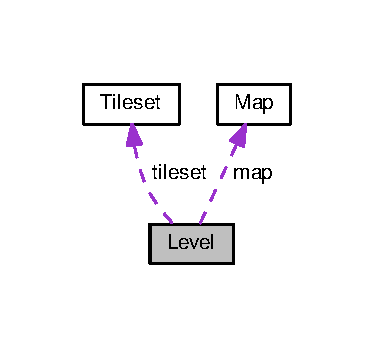
\includegraphics[width=180pt]{classLevel__coll__graph}
\end{center}
\end{figure}
\subsection*{Public Member Functions}
\begin{DoxyCompactItemize}
\item 
void {\bfseries create\+Level} (\hyperlink{classMap}{Map} m, \hyperlink{classTileset}{Tileset} t)\hypertarget{classLevel_a864fb9f328b7cf5be2a39e858e9681f5}{}\label{classLevel_a864fb9f328b7cf5be2a39e858e9681f5}

\item 
void {\bfseries create\+Level} (string filename, string name, string img, S\+D\+L\+\_\+\+Renderer $\ast$ren, int width, int height, int r, int count)\hypertarget{classLevel_a6346afdfc5eba1ce98254d5cdb39776d}{}\label{classLevel_a6346afdfc5eba1ce98254d5cdb39776d}

\item 
void {\bfseries create\+Level} (string filename, string name, string img, S\+D\+L\+\_\+\+Renderer $\ast$ren, int width, int height, int r, int rcount, int count)\hypertarget{classLevel_aaa9e17c51ed13c6a2b11ff04e3e4d81e}{}\label{classLevel_aaa9e17c51ed13c6a2b11ff04e3e4d81e}

\item 
void {\bfseries create\+Level} (string filename, int startid, string name, string img, S\+D\+L\+\_\+\+Renderer $\ast$ren, int width, int height, int r, int count)\hypertarget{classLevel_a698588721ec86ea8bc1002b58543ac14}{}\label{classLevel_a698588721ec86ea8bc1002b58543ac14}

\item 
void {\bfseries create\+Level} (string filename, int startid, string name, string img, S\+D\+L\+\_\+\+Renderer $\ast$ren, int width, int height, int r, int rcount, int count)\hypertarget{classLevel_af9b3321b7dff0ba6077ac43e9d49756d}{}\label{classLevel_af9b3321b7dff0ba6077ac43e9d49756d}

\item 
void {\bfseries set\+Map} (\hyperlink{classMap}{Map} m)\hypertarget{classLevel_a825b41113f6da7e1294f42f463f98a4c}{}\label{classLevel_a825b41113f6da7e1294f42f463f98a4c}

\item 
\hyperlink{classMap}{Map} {\bfseries set\+Map} (string filename)\hypertarget{classLevel_a97b3a35b145204905ad4bdb4c19e36c7}{}\label{classLevel_a97b3a35b145204905ad4bdb4c19e36c7}

\item 
\hyperlink{classMap}{Map} {\bfseries get\+Map} () const \hypertarget{classLevel_ae40b6bfd8916e65cbcd10790702b1782}{}\label{classLevel_ae40b6bfd8916e65cbcd10790702b1782}

\item 
void {\bfseries set\+Tileset} (\hyperlink{classTileset}{Tileset} t)\hypertarget{classLevel_a684434ce7be09c5956e6a93a08b5076f}{}\label{classLevel_a684434ce7be09c5956e6a93a08b5076f}

\item 
\hyperlink{classTileset}{Tileset} {\bfseries set\+Tileset} (string name, string img, S\+D\+L\+\_\+\+Renderer $\ast$ren, int width, int height, int r, int count)\hypertarget{classLevel_af2efc35f43fcfba60a0dd5a43e412c2e}{}\label{classLevel_af2efc35f43fcfba60a0dd5a43e412c2e}

\item 
\hyperlink{classTileset}{Tileset} {\bfseries set\+Tileset} (string name, string img, S\+D\+L\+\_\+\+Renderer $\ast$ren, int width, int height, int r, int rcount, int count)\hypertarget{classLevel_a6e1874e8e365179362e6caf3c60d707a}{}\label{classLevel_a6e1874e8e365179362e6caf3c60d707a}

\item 
\hyperlink{classTileset}{Tileset} {\bfseries set\+Tileset} (int startid, string name, string img, S\+D\+L\+\_\+\+Renderer $\ast$ren, int width, int height, int r, int count)\hypertarget{classLevel_ae735629e2ed290aa68545acb67ad3877}{}\label{classLevel_ae735629e2ed290aa68545acb67ad3877}

\item 
\hyperlink{classTileset}{Tileset} {\bfseries set\+Tileset} (int startid, string name, string img, S\+D\+L\+\_\+\+Renderer $\ast$ren, int width, int height, int r, int rcount, int count)\hypertarget{classLevel_a92388f78f651f7aea81d39f227c1cae3}{}\label{classLevel_a92388f78f651f7aea81d39f227c1cae3}

\item 
\hyperlink{classTileset}{Tileset} {\bfseries get\+Tileset} () const \hypertarget{classLevel_af6e51b47f493d8282b6648ec9e4054a3}{}\label{classLevel_af6e51b47f493d8282b6648ec9e4054a3}

\end{DoxyCompactItemize}
\subsection*{Private Attributes}
\begin{DoxyCompactItemize}
\item 
\hyperlink{classMap}{Map} {\bfseries map}\hypertarget{classLevel_acd59c9055fdd6c15b0a1adf6e451f0ba}{}\label{classLevel_acd59c9055fdd6c15b0a1adf6e451f0ba}

\item 
\hyperlink{classTileset}{Tileset} {\bfseries tileset}\hypertarget{classLevel_a7f2da1fccdb1b0dd6742649f3367324b}{}\label{classLevel_a7f2da1fccdb1b0dd6742649f3367324b}

\end{DoxyCompactItemize}


\subsection{Detailed Description}


Definition at line 7 of file level.\+h.



The documentation for this class was generated from the following files\+:\begin{DoxyCompactItemize}
\item 
level.\+h\item 
level.\+cpp\end{DoxyCompactItemize}

\hypertarget{classMap}{}\section{Map Class Reference}
\label{classMap}\index{Map@{Map}}


This class takes in a file and loads it in for the map.  




{\ttfamily \#include $<$map.\+h$>$}

\subsection*{Public Member Functions}
\begin{DoxyCompactItemize}
\item 
\mbox{\Hypertarget{classMap_a51e1c9c777bc6c4171707f1528a73dc6}\label{classMap_a51e1c9c777bc6c4171707f1528a73dc6}} 
void \hyperlink{classMap_a51e1c9c777bc6c4171707f1528a73dc6}{load\+Map} (string filename)
\begin{DoxyCompactList}\small\item\em Read in map file with given path to the file. \end{DoxyCompactList}\item 
\mbox{\Hypertarget{classMap_a4b4b995cd7b54aa9d8b87f353c0d88c5}\label{classMap_a4b4b995cd7b54aa9d8b87f353c0d88c5}} 
int \hyperlink{classMap_a4b4b995cd7b54aa9d8b87f353c0d88c5}{getX} () const
\begin{DoxyCompactList}\small\item\em Get the start x coordinate found in the file. \end{DoxyCompactList}\item 
\mbox{\Hypertarget{classMap_a0205e02d14a6112ae96cde67b87e2da2}\label{classMap_a0205e02d14a6112ae96cde67b87e2da2}} 
int \hyperlink{classMap_a0205e02d14a6112ae96cde67b87e2da2}{getY} () const
\begin{DoxyCompactList}\small\item\em Get the start y coordinate found in the file. \end{DoxyCompactList}\item 
\mbox{\Hypertarget{classMap_a0b54608da842cf193f6a6fb7838076f2}\label{classMap_a0b54608da842cf193f6a6fb7838076f2}} 
vector$<$ vector$<$ int $>$ $>$ \hyperlink{classMap_a0b54608da842cf193f6a6fb7838076f2}{get\+Map} () const
\begin{DoxyCompactList}\small\item\em Get the vector of integers found in the file. \end{DoxyCompactList}\end{DoxyCompactItemize}


\subsection{Detailed Description}
This class takes in a file and loads it in for the map. 

Definition at line 10 of file map.\+h.



The documentation for this class was generated from the following files\+:\begin{DoxyCompactItemize}
\item 
map.\+h\item 
map.\+cpp\end{DoxyCompactItemize}

\hypertarget{classObject}{}\section{Object Class Reference}
\label{classObject}\index{Object@{Object}}


Class for storing an image and the source and distination to display.  




{\ttfamily \#include $<$object.\+h$>$}



Inheritance diagram for Object\+:
% FIG 0


Collaboration diagram for Object\+:
% FIG 1
\subsection*{Public Member Functions}
\begin{DoxyCompactItemize}
\item 
void \hyperlink{classObject_a7f984ff2fb0c60b942a1018fc48417ae}{set\+Image} (string file, S\+D\+L\+\_\+\+Renderer $\ast$ren)\hypertarget{classObject_a7f984ff2fb0c60b942a1018fc48417ae}{}\label{classObject_a7f984ff2fb0c60b942a1018fc48417ae}

\begin{DoxyCompactList}\small\item\em Set the Objects image with a B\+MP image path and the renderer. \end{DoxyCompactList}\item 
\hyperlink{classImage}{Image} \hyperlink{classObject_a76748c591087e0a3c676daea6f257e08}{get\+Image} () const \hypertarget{classObject_a76748c591087e0a3c676daea6f257e08}{}\label{classObject_a76748c591087e0a3c676daea6f257e08}

\begin{DoxyCompactList}\small\item\em Get the \hyperlink{classObject}{Object}\textquotesingle{}s \hyperlink{classImage}{Image}. \end{DoxyCompactList}\item 
S\+D\+L\+\_\+\+Texture $\ast$ \hyperlink{classObject_af8ae0f74940285c54e90f19027bba3a7}{get\+Texture} ()\hypertarget{classObject_af8ae0f74940285c54e90f19027bba3a7}{}\label{classObject_af8ae0f74940285c54e90f19027bba3a7}

\begin{DoxyCompactList}\small\item\em Get the \hyperlink{classImage}{Image}\textquotesingle{}s texture. \end{DoxyCompactList}\item 
void \hyperlink{classObject_a094e6dc25b31cfac9d745869a878bd8b}{set\+Source} (double x, double y, int w, int h)\hypertarget{classObject_a094e6dc25b31cfac9d745869a878bd8b}{}\label{classObject_a094e6dc25b31cfac9d745869a878bd8b}

\begin{DoxyCompactList}\small\item\em Set the images source with the width, height, and x and y coordinates. \end{DoxyCompactList}\item 
void \hyperlink{classObject_a0ba46a30886b3d30e2b9a8a263b6c9b9}{set\+Dest} (int w, int h)\hypertarget{classObject_a0ba46a30886b3d30e2b9a8a263b6c9b9}{}\label{classObject_a0ba46a30886b3d30e2b9a8a263b6c9b9}

\begin{DoxyCompactList}\small\item\em Set the display destinations width and height. \end{DoxyCompactList}\item 
void \hyperlink{classObject_a9338eab393a21158dd0087b3b9d2e5e2}{set\+Dest} (int w, int h, double x, double y)\hypertarget{classObject_a9338eab393a21158dd0087b3b9d2e5e2}{}\label{classObject_a9338eab393a21158dd0087b3b9d2e5e2}

\begin{DoxyCompactList}\small\item\em Set the display destinations width, height, and x and y coordinates. \end{DoxyCompactList}\item 
void \hyperlink{classObject_a92a957d9f65d973c087367d26b358f0b}{set\+Dest\+Coord} (double x, double y)\hypertarget{classObject_a92a957d9f65d973c087367d26b358f0b}{}\label{classObject_a92a957d9f65d973c087367d26b358f0b}

\begin{DoxyCompactList}\small\item\em Set the display destinations x and y coordinates. \end{DoxyCompactList}\item 
S\+D\+L\+\_\+\+Rect \hyperlink{classObject_a411820194b7a02fcec714a51382c0c0c}{get\+Source} ()\hypertarget{classObject_a411820194b7a02fcec714a51382c0c0c}{}\label{classObject_a411820194b7a02fcec714a51382c0c0c}

\begin{DoxyCompactList}\small\item\em Get the S\+D\+L\+\_\+\+Rect of the Objects image source. \end{DoxyCompactList}\item 
S\+D\+L\+\_\+\+Rect \hyperlink{classObject_ab081a97a21c840bbcf3fd8ed3510f71d}{get\+Dest} ()\hypertarget{classObject_ab081a97a21c840bbcf3fd8ed3510f71d}{}\label{classObject_ab081a97a21c840bbcf3fd8ed3510f71d}

\begin{DoxyCompactList}\small\item\em Get the current S\+D\+L\+\_\+\+Rect for the Objects destination. \end{DoxyCompactList}\item 
S\+D\+L\+\_\+\+Rect \hyperlink{classObject_ad6363cce8614921f01b9ed9c1e068f65}{get\+Buff} ()\hypertarget{classObject_ad6363cce8614921f01b9ed9c1e068f65}{}\label{classObject_ad6363cce8614921f01b9ed9c1e068f65}

\begin{DoxyCompactList}\small\item\em Get the previous display destination. \end{DoxyCompactList}\item 
void \hyperlink{classObject_ab53b92a384c274bc1805eb50617d5117}{set\+Source} (S\+D\+L\+\_\+\+Rect s)\hypertarget{classObject_ab53b92a384c274bc1805eb50617d5117}{}\label{classObject_ab53b92a384c274bc1805eb50617d5117}

\begin{DoxyCompactList}\small\item\em Set the image source destination with an S\+D\+L\+\_\+\+Rect. \end{DoxyCompactList}\item 
void \hyperlink{classObject_a0edcf4141d5f6b86337597ecac4f8df2}{set\+Dest} (S\+D\+L\+\_\+\+Rect d)\hypertarget{classObject_a0edcf4141d5f6b86337597ecac4f8df2}{}\label{classObject_a0edcf4141d5f6b86337597ecac4f8df2}

\begin{DoxyCompactList}\small\item\em Set the \hyperlink{classObject}{Object}\textquotesingle{}s display destination with an S\+D\+L\+\_\+\+Rect. \end{DoxyCompactList}\item 
void \hyperlink{classObject_aa4a5d9d35931d9a0ad47557c3ca23ac7}{set\+Buff} (S\+D\+L\+\_\+\+Rect b)\hypertarget{classObject_aa4a5d9d35931d9a0ad47557c3ca23ac7}{}\label{classObject_aa4a5d9d35931d9a0ad47557c3ca23ac7}

\begin{DoxyCompactList}\small\item\em Set the object\textquotesingle{}s previous display destination with an S\+D\+L\+\_\+\+Rect. \end{DoxyCompactList}\item 
void \hyperlink{classObject_a63266f7fbaade4768bf6d60d0b313508}{set\+SX} (double x)\hypertarget{classObject_a63266f7fbaade4768bf6d60d0b313508}{}\label{classObject_a63266f7fbaade4768bf6d60d0b313508}

\begin{DoxyCompactList}\small\item\em Set the image sources x coordinate. \end{DoxyCompactList}\item 
void \hyperlink{classObject_a48c2da85369813e9bf1eb71eee579e8f}{set\+SY} (double y)\hypertarget{classObject_a48c2da85369813e9bf1eb71eee579e8f}{}\label{classObject_a48c2da85369813e9bf1eb71eee579e8f}

\begin{DoxyCompactList}\small\item\em Set the image sources y coordinate. \end{DoxyCompactList}\item 
void \hyperlink{classObject_a90577eaa8ea00ed7d01bf6829719322b}{set\+SW} (int w)\hypertarget{classObject_a90577eaa8ea00ed7d01bf6829719322b}{}\label{classObject_a90577eaa8ea00ed7d01bf6829719322b}

\begin{DoxyCompactList}\small\item\em Set the image sources width. \end{DoxyCompactList}\item 
void \hyperlink{classObject_a91800313b280d6812e2b374608172d7f}{set\+SH} (int h)\hypertarget{classObject_a91800313b280d6812e2b374608172d7f}{}\label{classObject_a91800313b280d6812e2b374608172d7f}

\begin{DoxyCompactList}\small\item\em Set the image sources height. \end{DoxyCompactList}\item 
void \hyperlink{classObject_a7c068c88758bf95a147b123ce52026a0}{set\+DX} (double x)\hypertarget{classObject_a7c068c88758bf95a147b123ce52026a0}{}\label{classObject_a7c068c88758bf95a147b123ce52026a0}

\begin{DoxyCompactList}\small\item\em Set the display destinations x coordinate. \end{DoxyCompactList}\item 
void \hyperlink{classObject_a9e7d9c484f3cdeac79edf6b1b13942d0}{set\+DY} (double y)\hypertarget{classObject_a9e7d9c484f3cdeac79edf6b1b13942d0}{}\label{classObject_a9e7d9c484f3cdeac79edf6b1b13942d0}

\begin{DoxyCompactList}\small\item\em Set the display destinations y coordinate. \end{DoxyCompactList}\item 
void \hyperlink{classObject_a7c9fcca4e1bab0097443557d02eaa498}{set\+DW} (int w)\hypertarget{classObject_a7c9fcca4e1bab0097443557d02eaa498}{}\label{classObject_a7c9fcca4e1bab0097443557d02eaa498}

\begin{DoxyCompactList}\small\item\em Set the display destinations width. \end{DoxyCompactList}\item 
void \hyperlink{classObject_a2c7a299d4311e4b2515022383f90b82a}{set\+DH} (int h)\hypertarget{classObject_a2c7a299d4311e4b2515022383f90b82a}{}\label{classObject_a2c7a299d4311e4b2515022383f90b82a}

\begin{DoxyCompactList}\small\item\em Set the display destinations height. \end{DoxyCompactList}\item 
double \hyperlink{classObject_a0f2d1703de76d3b7df5695962fe9dcc1}{get\+SX} ()\hypertarget{classObject_a0f2d1703de76d3b7df5695962fe9dcc1}{}\label{classObject_a0f2d1703de76d3b7df5695962fe9dcc1}

\begin{DoxyCompactList}\small\item\em Get the image sources x coordinate. \end{DoxyCompactList}\item 
double \hyperlink{classObject_a1ca9433993915dfb694d52c83494e73f}{get\+SY} ()\hypertarget{classObject_a1ca9433993915dfb694d52c83494e73f}{}\label{classObject_a1ca9433993915dfb694d52c83494e73f}

\begin{DoxyCompactList}\small\item\em Get the image sources y coordinate. \end{DoxyCompactList}\item 
double \hyperlink{classObject_aace84f90379d216d6f1e54b0aa4442d5}{get\+SW} ()\hypertarget{classObject_aace84f90379d216d6f1e54b0aa4442d5}{}\label{classObject_aace84f90379d216d6f1e54b0aa4442d5}

\begin{DoxyCompactList}\small\item\em Get the image sources width. \end{DoxyCompactList}\item 
double \hyperlink{classObject_a45fac8f64cae5bbc8566e69fb80037bf}{get\+SH} ()\hypertarget{classObject_a45fac8f64cae5bbc8566e69fb80037bf}{}\label{classObject_a45fac8f64cae5bbc8566e69fb80037bf}

\begin{DoxyCompactList}\small\item\em Get the image sources height. \end{DoxyCompactList}\item 
double \hyperlink{classObject_a16e291133d12358785e1bcc044615bcd}{get\+DX} ()\hypertarget{classObject_a16e291133d12358785e1bcc044615bcd}{}\label{classObject_a16e291133d12358785e1bcc044615bcd}

\begin{DoxyCompactList}\small\item\em Get the display destinations x coordinate. \end{DoxyCompactList}\item 
double \hyperlink{classObject_a6b011de1c1529d64b2cf3828f0450180}{get\+DY} ()\hypertarget{classObject_a6b011de1c1529d64b2cf3828f0450180}{}\label{classObject_a6b011de1c1529d64b2cf3828f0450180}

\begin{DoxyCompactList}\small\item\em Get the display destinations y coordinate. \end{DoxyCompactList}\item 
double \hyperlink{classObject_aa02be608cc4043a38675b93d69f5b42f}{get\+DW} ()\hypertarget{classObject_aa02be608cc4043a38675b93d69f5b42f}{}\label{classObject_aa02be608cc4043a38675b93d69f5b42f}

\begin{DoxyCompactList}\small\item\em Get the display destinations width. \end{DoxyCompactList}\item 
double \hyperlink{classObject_a9bb26c1b30e1a77a6ae4de340c4ab2f4}{get\+DH} ()\hypertarget{classObject_a9bb26c1b30e1a77a6ae4de340c4ab2f4}{}\label{classObject_a9bb26c1b30e1a77a6ae4de340c4ab2f4}

\begin{DoxyCompactList}\small\item\em Get the display destinations height. \end{DoxyCompactList}\item 
void \hyperlink{classObject_a660b00ecff522cd7dfef7b0f736456e6}{set\+Ang} (double a)\hypertarget{classObject_a660b00ecff522cd7dfef7b0f736456e6}{}\label{classObject_a660b00ecff522cd7dfef7b0f736456e6}

\begin{DoxyCompactList}\small\item\em Set the Objects angle. \end{DoxyCompactList}\item 
double \hyperlink{classObject_a9d6545d0250767ddb6e9d4c6fbf41d4b}{get\+Ang} ()\hypertarget{classObject_a9d6545d0250767ddb6e9d4c6fbf41d4b}{}\label{classObject_a9d6545d0250767ddb6e9d4c6fbf41d4b}

\begin{DoxyCompactList}\small\item\em Get the Objects angle. \end{DoxyCompactList}\item 
void \hyperlink{classObject_a31ef66bafcc755414112789c9231a8be}{move} (double mx, double my)\hypertarget{classObject_a31ef66bafcc755414112789c9231a8be}{}\label{classObject_a31ef66bafcc755414112789c9231a8be}

\begin{DoxyCompactList}\small\item\em Move the \hyperlink{classObject}{Object} x and y amount. \end{DoxyCompactList}\item 
void \hyperlink{classObject_a95af63b61c22ac2a8117742b9fa0efb5}{center} (int w, int h)\hypertarget{classObject_a95af63b61c22ac2a8117742b9fa0efb5}{}\label{classObject_a95af63b61c22ac2a8117742b9fa0efb5}

\begin{DoxyCompactList}\small\item\em Center the \hyperlink{classObject}{Object}\textquotesingle{}s destination by the given screens (or anythings) width and height. \end{DoxyCompactList}\item 
bool \hyperlink{classObject_a2a09d094befe949a0b879a62244de46e}{collidable} ()\hypertarget{classObject_a2a09d094befe949a0b879a62244de46e}{}\label{classObject_a2a09d094befe949a0b879a62244de46e}

\begin{DoxyCompactList}\small\item\em Check if the \hyperlink{classObject}{Object} is solid, or collidable. \end{DoxyCompactList}\item 
void \hyperlink{classObject_a470cdfc175b5fb0bd324a585ee5fce3f}{set\+Solid} (bool s)\hypertarget{classObject_a470cdfc175b5fb0bd324a585ee5fce3f}{}\label{classObject_a470cdfc175b5fb0bd324a585ee5fce3f}

\begin{DoxyCompactList}\small\item\em Set the \hyperlink{classObject}{Object} to be collidable/solid. \end{DoxyCompactList}\item 
bool \hyperlink{classObject_a5efbee91dd5bf04c6fb4bffef99ceba8}{get\+Solid} () const \hypertarget{classObject_a5efbee91dd5bf04c6fb4bffef99ceba8}{}\label{classObject_a5efbee91dd5bf04c6fb4bffef99ceba8}

\begin{DoxyCompactList}\small\item\em Check if the \hyperlink{classObject}{Object} is solid. \end{DoxyCompactList}\item 
int \hyperlink{classObject_a21238c368f570c14722cb00b74353732}{create\+New\+Frame\+Set} (int f\+Count, int r, int c, int w, int h)\hypertarget{classObject_a21238c368f570c14722cb00b74353732}{}\label{classObject_a21238c368f570c14722cb00b74353732}

\begin{DoxyCompactList}\small\item\em Create a new frameset with the given framecount for the set, the row to get the frameset from, the column to start at, and the width and height of each frame. Returns an int ID for the frameset. \end{DoxyCompactList}\item 
S\+D\+L\+\_\+\+Rect \hyperlink{classObject_a7a2350db0bae3e53ca9f928e08241159}{create\+New\+Frame} (int x, int y, int w, int h)\hypertarget{classObject_a7a2350db0bae3e53ca9f928e08241159}{}\label{classObject_a7a2350db0bae3e53ca9f928e08241159}

\begin{DoxyCompactList}\small\item\em Create a new frame with a given x and y coordinate and width and height. Automatically called from \hyperlink{classObject_a21238c368f570c14722cb00b74353732}{create\+New\+Frame\+Set()}. \end{DoxyCompactList}\item 
void \hyperlink{classObject_a061542647f10e3f30565ad9f56dc64c4}{set\+Cur\+Frame\+Set} (int fs)\hypertarget{classObject_a061542647f10e3f30565ad9f56dc64c4}{}\label{classObject_a061542647f10e3f30565ad9f56dc64c4}

\begin{DoxyCompactList}\small\item\em Set the current frameset with the given frameset ID from calling \hyperlink{classObject_a21238c368f570c14722cb00b74353732}{create\+New\+Frame\+Set()}. \end{DoxyCompactList}\item 
void \hyperlink{classObject_aef259fb0225c8995ec2c0ebe04c98cd9}{set\+Cur\+Frame} (int f)\hypertarget{classObject_aef259fb0225c8995ec2c0ebe04c98cd9}{}\label{classObject_aef259fb0225c8995ec2c0ebe04c98cd9}

\begin{DoxyCompactList}\small\item\em Set current frame in the frameset. \end{DoxyCompactList}\item 
void \hyperlink{classObject_a2c123e98f36c3779f5172afefacbf69c}{next\+Frame} ()\hypertarget{classObject_a2c123e98f36c3779f5172afefacbf69c}{}\label{classObject_a2c123e98f36c3779f5172afefacbf69c}

\begin{DoxyCompactList}\small\item\em Change to the next frame. If it reaches its end, it restarts. Called in \hyperlink{classObject_a061542647f10e3f30565ad9f56dc64c4}{set\+Cur\+Frame\+Set()}. \end{DoxyCompactList}\item 
void \hyperlink{classObject_ab2a55c6e2908f754992cc1c281b01be8}{reset\+Frame\+Set} ()\hypertarget{classObject_ab2a55c6e2908f754992cc1c281b01be8}{}\label{classObject_ab2a55c6e2908f754992cc1c281b01be8}

\begin{DoxyCompactList}\small\item\em Set current frame to the beginning. Called in \hyperlink{classObject_a2c123e98f36c3779f5172afefacbf69c}{next\+Frame()} when it has reached its end. \end{DoxyCompactList}\item 
int \hyperlink{classObject_a3de9dd15d8ba28785284bccd2cfc406c}{get\+Cur\+Frame\+Set} () const \hypertarget{classObject_a3de9dd15d8ba28785284bccd2cfc406c}{}\label{classObject_a3de9dd15d8ba28785284bccd2cfc406c}

\begin{DoxyCompactList}\small\item\em Get the current frameset. \end{DoxyCompactList}\item 
int \hyperlink{classObject_a21b245ca66eaee32f3d942759c0de620}{get\+Cur\+Frame} () const \hypertarget{classObject_a21b245ca66eaee32f3d942759c0de620}{}\label{classObject_a21b245ca66eaee32f3d942759c0de620}

\begin{DoxyCompactList}\small\item\em Get the current frame. \end{DoxyCompactList}\end{DoxyCompactItemize}
\subsection*{Private Attributes}
\begin{DoxyCompactItemize}
\item 
\hyperlink{classImage}{Image} \hyperlink{classObject_a78cbd7ab6622400668b41dd6b32f2f4d}{img}\hypertarget{classObject_a78cbd7ab6622400668b41dd6b32f2f4d}{}\label{classObject_a78cbd7ab6622400668b41dd6b32f2f4d}

\begin{DoxyCompactList}\small\item\em The Objects image. \end{DoxyCompactList}\item 
S\+D\+L\+\_\+\+Rect \hyperlink{classObject_ac2bf39eb033cf8c8fc9220d607842dbe}{rect}\hypertarget{classObject_ac2bf39eb033cf8c8fc9220d607842dbe}{}\label{classObject_ac2bf39eb033cf8c8fc9220d607842dbe}

\begin{DoxyCompactList}\small\item\em The images source. \end{DoxyCompactList}\item 
S\+D\+L\+\_\+\+Rect \hyperlink{classObject_a65a8afd007a1a0dbd67d6997b33b271b}{dest}\hypertarget{classObject_a65a8afd007a1a0dbd67d6997b33b271b}{}\label{classObject_a65a8afd007a1a0dbd67d6997b33b271b}

\begin{DoxyCompactList}\small\item\em The display destination. \end{DoxyCompactList}\item 
S\+D\+L\+\_\+\+Rect \hyperlink{classObject_adff14724f0adf5774e2241eabe7965c8}{buff}\hypertarget{classObject_adff14724f0adf5774e2241eabe7965c8}{}\label{classObject_adff14724f0adf5774e2241eabe7965c8}

\begin{DoxyCompactList}\small\item\em Previous display destination. \end{DoxyCompactList}\item 
double \hyperlink{classObject_aa08efab6c2c6898b1d0d7103076d8674}{angle}\hypertarget{classObject_aa08efab6c2c6898b1d0d7103076d8674}{}\label{classObject_aa08efab6c2c6898b1d0d7103076d8674}

\begin{DoxyCompactList}\small\item\em Angle to be displayed. \end{DoxyCompactList}\item 
bool \hyperlink{classObject_a4cb593f1e74999419dd38fceaa8ad474}{solid}\hypertarget{classObject_a4cb593f1e74999419dd38fceaa8ad474}{}\label{classObject_a4cb593f1e74999419dd38fceaa8ad474}

\begin{DoxyCompactList}\small\item\em Boolean for if the \hyperlink{classObject}{Object} is collidable/solid. \end{DoxyCompactList}\item 
vector$<$ vector$<$ S\+D\+L\+\_\+\+Rect $>$ $>$ \hyperlink{classObject_a6dea9199db9c71cadb54202448a85fc4}{frameset}\hypertarget{classObject_a6dea9199db9c71cadb54202448a85fc4}{}\label{classObject_a6dea9199db9c71cadb54202448a85fc4}

\begin{DoxyCompactList}\small\item\em 2D vector of framesets that store frames. \end{DoxyCompactList}\item 
int \hyperlink{classObject_a2a137e8005d1923f22d90d965b2d11f0}{cur\+Frame\+Set}\hypertarget{classObject_a2a137e8005d1923f22d90d965b2d11f0}{}\label{classObject_a2a137e8005d1923f22d90d965b2d11f0}

\begin{DoxyCompactList}\small\item\em Current frameset. \end{DoxyCompactList}\item 
int \hyperlink{classObject_aac9e198e982b2fb98d94ee66483d2880}{cur\+Frame}\hypertarget{classObject_aac9e198e982b2fb98d94ee66483d2880}{}\label{classObject_aac9e198e982b2fb98d94ee66483d2880}

\begin{DoxyCompactList}\small\item\em Current frame. \end{DoxyCompactList}\end{DoxyCompactItemize}


\subsection{Detailed Description}
Class for storing an image and the source and distination to display. 

Definition at line 10 of file object.\+h.



The documentation for this class was generated from the following files\+:\begin{DoxyCompactItemize}
\item 
object.\+h\item 
object.\+cpp\end{DoxyCompactItemize}

\hypertarget{classPhysics}{}\section{Physics Class Reference}
\label{classPhysics}\index{Physics@{Physics}}


Class for doing physics functions.  




{\ttfamily \#include $<$physics-\/tmp.\+h$>$}

\subsection*{Public Member Functions}
\begin{DoxyCompactItemize}
\item 
\hyperlink{classObject}{Object} \hyperlink{classPhysics_a8e53f9bf088c0d4f208b3c2029d69ab2}{move\+Towards} (\hyperlink{classObject}{Object} cur, \hyperlink{classObject}{Object} des)\hypertarget{classPhysics_a8e53f9bf088c0d4f208b3c2029d69ab2}{}\label{classPhysics_a8e53f9bf088c0d4f208b3c2029d69ab2}

\begin{DoxyCompactList}\small\item\em Returns modified first \hyperlink{classObject}{Object} that is moving towards the second object (I T\+H\+I\+NK). \end{DoxyCompactList}\end{DoxyCompactItemize}


\subsection{Detailed Description}
Class for doing physics functions. 

Definition at line 23 of file physics-\/tmp.\+h.



The documentation for this class was generated from the following files\+:\begin{DoxyCompactItemize}
\item 
physics-\/tmp.\+h\item 
physics-\/tmp.\+cpp\end{DoxyCompactItemize}

\hypertarget{classStage}{}\section{Stage Class Reference}
\label{classStage}\index{Stage@{Stage}}


The \hyperlink{classStage}{Stage} class stores a \hyperlink{classMap}{Map} and \hyperlink{classTileset}{Tileset}.  




{\ttfamily \#include $<$stage.\+h$>$}

\subsection*{Public Member Functions}
\begin{DoxyCompactItemize}
\item 
\mbox{\Hypertarget{classStage_a716561c7b2b148b67e7cf4952bae937b}\label{classStage_a716561c7b2b148b67e7cf4952bae937b}} 
void \hyperlink{classStage_a716561c7b2b148b67e7cf4952bae937b}{create\+Stage} (\hyperlink{classMap}{Map} m, \hyperlink{classTileset}{Tileset} t)
\begin{DoxyCompactList}\small\item\em Create a stage by passing in a \hyperlink{classMap}{Map} and \hyperlink{classTileset}{Tileset}. \end{DoxyCompactList}\item 
\mbox{\Hypertarget{classStage_ad552bc548e34ff668944a6fc20b2aa0d}\label{classStage_ad552bc548e34ff668944a6fc20b2aa0d}} 
void \hyperlink{classStage_ad552bc548e34ff668944a6fc20b2aa0d}{create\+Stage} (string filename, string name, string img, S\+D\+L\+\_\+\+Renderer $\ast$ren, int width, int height, int r, int count)
\begin{DoxyCompactList}\small\item\em Create a stage by passing in the maps file, a name for the tiles, file of the tile image, the renderer, width and height of a tile, what row of the image the tiles are onem and how many tiles there are. \end{DoxyCompactList}\item 
\mbox{\Hypertarget{classStage_a871e4913cf2566a1a3a21c9d2e962648}\label{classStage_a871e4913cf2566a1a3a21c9d2e962648}} 
void {\bfseries create\+Stage} (string filename, string name, string img, S\+D\+L\+\_\+\+Renderer $\ast$ren, int width, int height, int r, int rcount, int count)
\item 
\mbox{\Hypertarget{classStage_a8ab003560188a4004ee497fd23692833}\label{classStage_a8ab003560188a4004ee497fd23692833}} 
void {\bfseries create\+Stage} (string filename, int startid, string name, string img, S\+D\+L\+\_\+\+Renderer $\ast$ren, int width, int height, int r, int count)
\item 
\mbox{\Hypertarget{classStage_a2d9071d75c90883539cd303c128a6b7d}\label{classStage_a2d9071d75c90883539cd303c128a6b7d}} 
void {\bfseries create\+Stage} (string filename, int startid, string name, string img, S\+D\+L\+\_\+\+Renderer $\ast$ren, int width, int height, int r, int rcount, int count)
\item 
\mbox{\Hypertarget{classStage_a47a215785ca66ffae354c350aee1800e}\label{classStage_a47a215785ca66ffae354c350aee1800e}} 
void \hyperlink{classStage_a47a215785ca66ffae354c350aee1800e}{set\+Map} (\hyperlink{classMap}{Map} m)
\begin{DoxyCompactList}\small\item\em Set the \hyperlink{classMap}{Map} by passing in a \hyperlink{classMap}{Map}. \end{DoxyCompactList}\item 
\mbox{\Hypertarget{classStage_a11b7cabe85812fda7513d14d6b21ff6a}\label{classStage_a11b7cabe85812fda7513d14d6b21ff6a}} 
\hyperlink{classMap}{Map} \hyperlink{classStage_a11b7cabe85812fda7513d14d6b21ff6a}{set\+Map} (string filename)
\begin{DoxyCompactList}\small\item\em Load in a new map by passing in the map file. \end{DoxyCompactList}\item 
\mbox{\Hypertarget{classStage_a9f906d6b347432ddeee8894031a2c981}\label{classStage_a9f906d6b347432ddeee8894031a2c981}} 
\hyperlink{classMap}{Map} \hyperlink{classStage_a9f906d6b347432ddeee8894031a2c981}{get\+Map} () const
\begin{DoxyCompactList}\small\item\em Get the \hyperlink{classMap}{Map}. \end{DoxyCompactList}\item 
\mbox{\Hypertarget{classStage_a63a19b471f7c54d68f3f7e4419eca8ac}\label{classStage_a63a19b471f7c54d68f3f7e4419eca8ac}} 
void \hyperlink{classStage_a63a19b471f7c54d68f3f7e4419eca8ac}{set\+Tileset} (\hyperlink{classTileset}{Tileset} t)
\begin{DoxyCompactList}\small\item\em Set the \hyperlink{classTileset}{Tileset} with a given \hyperlink{classTileset}{Tileset}. \end{DoxyCompactList}\item 
\mbox{\Hypertarget{classStage_ab62ad01c46da0337c294c4790020306f}\label{classStage_ab62ad01c46da0337c294c4790020306f}} 
\hyperlink{classTileset}{Tileset} {\bfseries set\+Tileset} (string name, string img, S\+D\+L\+\_\+\+Renderer $\ast$ren, int width, int height, int r, int count)
\item 
\mbox{\Hypertarget{classStage_a6e71c30197676d98a4a5694ad8b5a733}\label{classStage_a6e71c30197676d98a4a5694ad8b5a733}} 
\hyperlink{classTileset}{Tileset} {\bfseries set\+Tileset} (string name, string img, S\+D\+L\+\_\+\+Renderer $\ast$ren, int width, int height, int r, int rcount, int count)
\item 
\mbox{\Hypertarget{classStage_ab90d4d0315e6991f2ed8216b6c804339}\label{classStage_ab90d4d0315e6991f2ed8216b6c804339}} 
\hyperlink{classTileset}{Tileset} {\bfseries set\+Tileset} (int startid, string name, string img, S\+D\+L\+\_\+\+Renderer $\ast$ren, int width, int height, int r, int count)
\item 
\mbox{\Hypertarget{classStage_a42ee2fbdb79971f90984f603fcad54d6}\label{classStage_a42ee2fbdb79971f90984f603fcad54d6}} 
\hyperlink{classTileset}{Tileset} {\bfseries set\+Tileset} (int startid, string name, string img, S\+D\+L\+\_\+\+Renderer $\ast$ren, int width, int height, int r, int rcount, int count)
\item 
\mbox{\Hypertarget{classStage_ab4df60dd0fa777ec19ff13056a17842a}\label{classStage_ab4df60dd0fa777ec19ff13056a17842a}} 
\hyperlink{classTileset}{Tileset} \hyperlink{classStage_ab4df60dd0fa777ec19ff13056a17842a}{get\+Tileset} () const
\begin{DoxyCompactList}\small\item\em Get the \hyperlink{classTileset}{Tileset}. \end{DoxyCompactList}\end{DoxyCompactItemize}


\subsection{Detailed Description}
The \hyperlink{classStage}{Stage} class stores a \hyperlink{classMap}{Map} and \hyperlink{classTileset}{Tileset}. 

Definition at line 8 of file stage.\+h.



The documentation for this class was generated from the following files\+:\begin{DoxyCompactItemize}
\item 
stage.\+h\item 
stage.\+cpp\end{DoxyCompactItemize}

\hypertarget{classTile}{}\section{Tile Class Reference}
\label{classTile}\index{Tile@{Tile}}


An \hyperlink{classObject}{Object} class that stores the a tile value and name.  




{\ttfamily \#include $<$tile.\+h$>$}



Inheritance diagram for Tile\+:\nopagebreak
\begin{figure}[H]
\begin{center}
\leavevmode
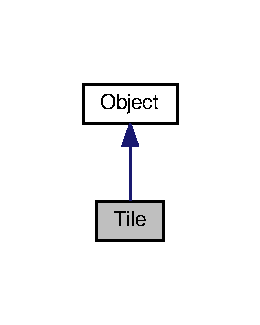
\includegraphics[width=125pt]{classTile__inherit__graph}
\end{center}
\end{figure}


Collaboration diagram for Tile\+:\nopagebreak
\begin{figure}[H]
\begin{center}
\leavevmode
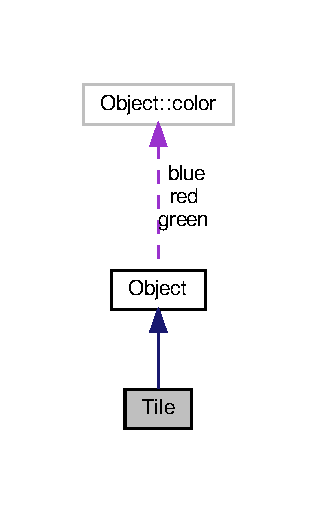
\includegraphics[width=125pt]{classTile__coll__graph}
\end{center}
\end{figure}
\subsection*{Public Member Functions}
\begin{DoxyCompactItemize}
\item 
void \hyperlink{classTile_ae3d9e4ace265389dd0e0cf3d62ad6ff3}{set\+Value} (int v)\hypertarget{classTile_ae3d9e4ace265389dd0e0cf3d62ad6ff3}{}\label{classTile_ae3d9e4ace265389dd0e0cf3d62ad6ff3}

\begin{DoxyCompactList}\small\item\em Set value of the tile. This is used when reading from a map file, etc. \end{DoxyCompactList}\item 
int \hyperlink{classTile_aa426a6476fcf257bd0f79da4c3ed06aa}{get\+Value} () const \hypertarget{classTile_aa426a6476fcf257bd0f79da4c3ed06aa}{}\label{classTile_aa426a6476fcf257bd0f79da4c3ed06aa}

\begin{DoxyCompactList}\small\item\em Get the value of the tile. \end{DoxyCompactList}\item 
void {\bfseries set\+Solid} ()\hypertarget{classTile_a3deac8e6d0ebd7b8352248201d264c38}{}\label{classTile_a3deac8e6d0ebd7b8352248201d264c38}

\item 
void {\bfseries set\+Passable} ()\hypertarget{classTile_a067099478c20b3f2fb56bc1c042a1e4e}{}\label{classTile_a067099478c20b3f2fb56bc1c042a1e4e}

\item 
bool {\bfseries is\+Solid} () const \hypertarget{classTile_a8e67a56637124f73f3da572178dd4838}{}\label{classTile_a8e67a56637124f73f3da572178dd4838}

\end{DoxyCompactItemize}
\subsection*{Private Attributes}
\begin{DoxyCompactItemize}
\item 
int \hyperlink{classTile_abc4813aabaaf0451b10bb45ed713bc7e}{value}\hypertarget{classTile_abc4813aabaaf0451b10bb45ed713bc7e}{}\label{classTile_abc4813aabaaf0451b10bb45ed713bc7e}

\begin{DoxyCompactList}\small\item\em Tiles value. Used for reading from a map file, etc. \end{DoxyCompactList}\item 
bool {\bfseries solid}\hypertarget{classTile_a9eec63370c6138ac19a5b48d1f32f855}{}\label{classTile_a9eec63370c6138ac19a5b48d1f32f855}

\end{DoxyCompactItemize}


\subsection{Detailed Description}
An \hyperlink{classObject}{Object} class that stores the a tile value and name. 

Definition at line 7 of file tile.\+h.



The documentation for this class was generated from the following files\+:\begin{DoxyCompactItemize}
\item 
tile.\+h\item 
tile.\+cpp\end{DoxyCompactItemize}

\hypertarget{classTileset}{}\section{Tileset Class Reference}
\label{classTileset}\index{Tileset@{Tileset}}


Class for loading in multiple Tiles.  




{\ttfamily \#include $<$arch.\+h$>$}

\subsection*{Public Member Functions}
\begin{DoxyCompactItemize}
\item 
vector$<$ \hyperlink{classTile}{Tile} $>$ {\bfseries get\+Tileset} () const \hypertarget{classTileset_ae5f7859d69952b223bdb322796bcc9f2}{}\label{classTileset_ae5f7859d69952b223bdb322796bcc9f2}

\item 
S\+D\+L\+\_\+\+Rect {\bfseries get\+Frame} (int i)\hypertarget{classTileset_aefa962edb9c573aca7327387ba6be0b1}{}\label{classTileset_aefa962edb9c573aca7327387ba6be0b1}

\item 
vector$<$ \hyperlink{classTile}{Tile} $>$ \hyperlink{classTileset_ad11cd044d9a2907003fee3baacba86e7}{create} (string name, string img, S\+D\+L\+\_\+\+Renderer $\ast$ren, int width, int height, int r, int count)\hypertarget{classTileset_ad11cd044d9a2907003fee3baacba86e7}{}\label{classTileset_ad11cd044d9a2907003fee3baacba86e7}

\begin{DoxyCompactList}\small\item\em Load in a map file with the name for all the tiles, the path to the map file, path to the tileset image, the S\+DL renderer, width and height of a tile, row to begin from on the image, how many tiles there are in the image. \end{DoxyCompactList}\item 
vector$<$ \hyperlink{classTile}{Tile} $>$ \hyperlink{classTileset_a1435c7ce70c5aa6da6388762971917aa}{create} (string name, string img, S\+D\+L\+\_\+\+Renderer $\ast$ren, int width, int height, int r, int rcount, int count)\hypertarget{classTileset_a1435c7ce70c5aa6da6388762971917aa}{}\label{classTileset_a1435c7ce70c5aa6da6388762971917aa}

\begin{DoxyCompactList}\small\item\em Load a map with a given name for the tiles, the file path to the map, the path to the tileset image, S\+DL renderer, width and height of a tile, row to begin on in the image, how many tiles on a certain row in the image, total amount of tiles in the image. \end{DoxyCompactList}\item 
vector$<$ \hyperlink{classTile}{Tile} $>$ \hyperlink{classTileset_a9d93cb00fc20938748075d94be118ed6}{create} (int startid, string name, string img, S\+D\+L\+\_\+\+Renderer $\ast$ren, int width, int height, int r, int count)\hypertarget{classTileset_a9d93cb00fc20938748075d94be118ed6}{}\label{classTileset_a9d93cb00fc20938748075d94be118ed6}

\begin{DoxyCompactList}\small\item\em Load in a map file with the name for all the tiles, the path to the map file, path to the tileset image, the S\+DL renderer, width and height of a tile, row to begin from on the image, how many tiles there are in the image. \end{DoxyCompactList}\item 
vector$<$ \hyperlink{classTile}{Tile} $>$ \hyperlink{classTileset_a7671c66fd7dfd4cf62524a5d518afbe6}{create} (int startid, string name, string img, S\+D\+L\+\_\+\+Renderer $\ast$ren, int width, int height, int r, int rcount, int count)\hypertarget{classTileset_a7671c66fd7dfd4cf62524a5d518afbe6}{}\label{classTileset_a7671c66fd7dfd4cf62524a5d518afbe6}

\begin{DoxyCompactList}\small\item\em Load a map with a given name for the tiles, the file path to the map, the path to the tileset image, S\+DL renderer, width and height of a tile, row to begin on in the image, how many tiles on a certain row in the image, total amount of tiles in the image. \end{DoxyCompactList}\item 
void \hyperlink{classTileset_a26acaabd06601aba2e277fdd2b750fc7}{add\+Tile} (\hyperlink{classTile}{Tile} t)\hypertarget{classTileset_a26acaabd06601aba2e277fdd2b750fc7}{}\label{classTileset_a26acaabd06601aba2e277fdd2b750fc7}

\begin{DoxyCompactList}\small\item\em Push \hyperlink{classTile}{Tile} in tile with given \hyperlink{classTile}{Tile}. \end{DoxyCompactList}\item 
\hyperlink{classTile}{Tile} \hyperlink{classTileset_aea4085286f450afdb53b22c917a77cba}{add\+Tile} (string name, string file, S\+D\+L\+\_\+\+Renderer $\ast$ren, int value, int r, int c, int width, int height)\hypertarget{classTileset_aea4085286f450afdb53b22c917a77cba}{}\label{classTileset_aea4085286f450afdb53b22c917a77cba}

\begin{DoxyCompactList}\small\item\em Generate and push \hyperlink{classTile}{Tile} with tile name, path tot he tile image, S\+DL renderer, tile value, row and columg the tile as on in the image, the tiles width and height. \end{DoxyCompactList}\item 
\hyperlink{classTile}{Tile} \hyperlink{classTileset_af8022d2b4129de86c132172ac8ce23a5}{add\+Tile} (string name, string file, S\+D\+L\+\_\+\+Renderer $\ast$ren, int value, int width, int height)\hypertarget{classTileset_af8022d2b4129de86c132172ac8ce23a5}{}\label{classTileset_af8022d2b4129de86c132172ac8ce23a5}

\begin{DoxyCompactList}\small\item\em Generate and push \hyperlink{classTile}{Tile} with a given name, path to image file, S\+DL renderer, given value, and tile width and height. \end{DoxyCompactList}\item 
\hyperlink{classTile}{Tile} \hyperlink{classTileset_adc54ffeda362f79668abb0bad2f73296}{add\+Tile} (string name, string file, S\+D\+L\+\_\+\+Renderer $\ast$ren, int value, int size)\hypertarget{classTileset_adc54ffeda362f79668abb0bad2f73296}{}\label{classTileset_adc54ffeda362f79668abb0bad2f73296}

\begin{DoxyCompactList}\small\item\em Generate and push \hyperlink{classTile}{Tile} with a given name, path to the image, S\+DL renderer, value, and size (used for width and height). \end{DoxyCompactList}\item 
void \hyperlink{classTileset_ab1dab8dd83a80e5d49dcdb95f9841898}{set\+Angle} (int ang)\hypertarget{classTileset_ab1dab8dd83a80e5d49dcdb95f9841898}{}\label{classTileset_ab1dab8dd83a80e5d49dcdb95f9841898}

\begin{DoxyCompactList}\small\item\em Set the angle of all the tiles. Calls push\+Ang(). \end{DoxyCompactList}\item 
void {\bfseries set\+Solid} ()\hypertarget{classTileset_a87978787ae2529b915c0436b5872dd48}{}\label{classTileset_a87978787ae2529b915c0436b5872dd48}

\item 
void {\bfseries set\+Solid} (int t)\hypertarget{classTileset_aa4dd63b2c6422ed5a9b7d772963fe255}{}\label{classTileset_aa4dd63b2c6422ed5a9b7d772963fe255}

\item 
void {\bfseries set\+Solid} (int s, int e)\hypertarget{classTileset_a6d40a14146a3dedd0217a412a66f4c9a}{}\label{classTileset_a6d40a14146a3dedd0217a412a66f4c9a}

\item 
void {\bfseries set\+Passable} ()\hypertarget{classTileset_a9fc3756317f238121769629ea20a9849}{}\label{classTileset_a9fc3756317f238121769629ea20a9849}

\item 
void {\bfseries set\+Passable} (int t)\hypertarget{classTileset_a231401092d65e28b7dea12e97e3232ad}{}\label{classTileset_a231401092d65e28b7dea12e97e3232ad}

\item 
void {\bfseries set\+Passable} (int s, int e)\hypertarget{classTileset_a84b12096b06c7162ca4bb9058a232d21}{}\label{classTileset_a84b12096b06c7162ca4bb9058a232d21}

\item 
void {\bfseries set\+Name} (string n, int id)\hypertarget{classTileset_ad5f3a60a84cec25c6e11856a7cd36d84}{}\label{classTileset_ad5f3a60a84cec25c6e11856a7cd36d84}

\item 
vector$<$ \hyperlink{classTile}{Tile} $>$ {\bfseries get\+Tileset} () const \hypertarget{classTileset_ae5f7859d69952b223bdb322796bcc9f2}{}\label{classTileset_ae5f7859d69952b223bdb322796bcc9f2}

\item 
S\+D\+L\+\_\+\+Rect {\bfseries get\+Frame} (int i)\hypertarget{classTileset_aefa962edb9c573aca7327387ba6be0b1}{}\label{classTileset_aefa962edb9c573aca7327387ba6be0b1}

\item 
vector$<$ \hyperlink{classTile}{Tile} $>$ \hyperlink{classTileset_a98c6192618c41b2083ff4c9224c6830d}{create} (string name, string img, S\+D\+L\+\_\+\+Renderer $\ast$ren, int width, int height, int r, int count)\hypertarget{classTileset_a98c6192618c41b2083ff4c9224c6830d}{}\label{classTileset_a98c6192618c41b2083ff4c9224c6830d}

\begin{DoxyCompactList}\small\item\em Load in a map file with the name for all the tiles, the path to the map file, path to the tileset image, the S\+DL renderer, width and height of a tile, row to begin from on the image, how many tiles there are in the image. \end{DoxyCompactList}\item 
vector$<$ \hyperlink{classTile}{Tile} $>$ \hyperlink{classTileset_af0fe3b9f21336f475f2763c9ea7c4a05}{create} (string name, string img, S\+D\+L\+\_\+\+Renderer $\ast$ren, int width, int height, int r, int rcount, int count)\hypertarget{classTileset_af0fe3b9f21336f475f2763c9ea7c4a05}{}\label{classTileset_af0fe3b9f21336f475f2763c9ea7c4a05}

\begin{DoxyCompactList}\small\item\em Load a map with a given name for the tiles, the file path to the map, the path to the tileset image, S\+DL renderer, width and height of a tile, row to begin on in the image, how many tiles on a certain row in the image, total amount of tiles in the image. \end{DoxyCompactList}\item 
vector$<$ \hyperlink{classTile}{Tile} $>$ \hyperlink{classTileset_aa9e6d07ce652af578d49d6415461d692}{create} (int startid, string name, string img, S\+D\+L\+\_\+\+Renderer $\ast$ren, int width, int height, int r, int count)\hypertarget{classTileset_aa9e6d07ce652af578d49d6415461d692}{}\label{classTileset_aa9e6d07ce652af578d49d6415461d692}

\begin{DoxyCompactList}\small\item\em Load in a map file with the name for all the tiles, the path to the map file, path to the tileset image, the S\+DL renderer, width and height of a tile, row to begin from on the image, how many tiles there are in the image. \end{DoxyCompactList}\item 
vector$<$ \hyperlink{classTile}{Tile} $>$ \hyperlink{classTileset_ae11e3dc2ff393646e68de707f47c71ea}{create} (int startid, string name, string img, S\+D\+L\+\_\+\+Renderer $\ast$ren, int width, int height, int r, int rcount, int count)\hypertarget{classTileset_ae11e3dc2ff393646e68de707f47c71ea}{}\label{classTileset_ae11e3dc2ff393646e68de707f47c71ea}

\begin{DoxyCompactList}\small\item\em Load a map with a given name for the tiles, the file path to the map, the path to the tileset image, S\+DL renderer, width and height of a tile, row to begin on in the image, how many tiles on a certain row in the image, total amount of tiles in the image. \end{DoxyCompactList}\item 
void \hyperlink{classTileset_a26acaabd06601aba2e277fdd2b750fc7}{add\+Tile} (\hyperlink{classTile}{Tile} t)\hypertarget{classTileset_a26acaabd06601aba2e277fdd2b750fc7}{}\label{classTileset_a26acaabd06601aba2e277fdd2b750fc7}

\begin{DoxyCompactList}\small\item\em Push \hyperlink{classTile}{Tile} in tile with given \hyperlink{classTile}{Tile}. \end{DoxyCompactList}\item 
\hyperlink{classTile}{Tile} \hyperlink{classTileset_aea4085286f450afdb53b22c917a77cba}{add\+Tile} (string name, string file, S\+D\+L\+\_\+\+Renderer $\ast$ren, int value, int r, int c, int width, int height)\hypertarget{classTileset_aea4085286f450afdb53b22c917a77cba}{}\label{classTileset_aea4085286f450afdb53b22c917a77cba}

\begin{DoxyCompactList}\small\item\em Generate and push \hyperlink{classTile}{Tile} with tile name, path tot he tile image, S\+DL renderer, tile value, row and columg the tile as on in the image, the tiles width and height. \end{DoxyCompactList}\item 
\hyperlink{classTile}{Tile} \hyperlink{classTileset_af8022d2b4129de86c132172ac8ce23a5}{add\+Tile} (string name, string file, S\+D\+L\+\_\+\+Renderer $\ast$ren, int value, int width, int height)\hypertarget{classTileset_af8022d2b4129de86c132172ac8ce23a5}{}\label{classTileset_af8022d2b4129de86c132172ac8ce23a5}

\begin{DoxyCompactList}\small\item\em Generate and push \hyperlink{classTile}{Tile} with a given name, path to image file, S\+DL renderer, given value, and tile width and height. \end{DoxyCompactList}\item 
\hyperlink{classTile}{Tile} \hyperlink{classTileset_adc54ffeda362f79668abb0bad2f73296}{add\+Tile} (string name, string file, S\+D\+L\+\_\+\+Renderer $\ast$ren, int value, int size)\hypertarget{classTileset_adc54ffeda362f79668abb0bad2f73296}{}\label{classTileset_adc54ffeda362f79668abb0bad2f73296}

\begin{DoxyCompactList}\small\item\em Generate and push \hyperlink{classTile}{Tile} with a given name, path to the image, S\+DL renderer, value, and size (used for width and height). \end{DoxyCompactList}\item 
void \hyperlink{classTileset_ab1dab8dd83a80e5d49dcdb95f9841898}{set\+Angle} (int ang)\hypertarget{classTileset_ab1dab8dd83a80e5d49dcdb95f9841898}{}\label{classTileset_ab1dab8dd83a80e5d49dcdb95f9841898}

\begin{DoxyCompactList}\small\item\em Set the angle of all the tiles. Calls push\+Ang(). \end{DoxyCompactList}\item 
void {\bfseries set\+Solid} ()\hypertarget{classTileset_a87978787ae2529b915c0436b5872dd48}{}\label{classTileset_a87978787ae2529b915c0436b5872dd48}

\item 
void {\bfseries set\+Solid} (int t)\hypertarget{classTileset_aa4dd63b2c6422ed5a9b7d772963fe255}{}\label{classTileset_aa4dd63b2c6422ed5a9b7d772963fe255}

\item 
void {\bfseries set\+Solid} (int s, int e)\hypertarget{classTileset_a6d40a14146a3dedd0217a412a66f4c9a}{}\label{classTileset_a6d40a14146a3dedd0217a412a66f4c9a}

\item 
void {\bfseries set\+Passable} ()\hypertarget{classTileset_a9fc3756317f238121769629ea20a9849}{}\label{classTileset_a9fc3756317f238121769629ea20a9849}

\item 
void {\bfseries set\+Passable} (int t)\hypertarget{classTileset_a231401092d65e28b7dea12e97e3232ad}{}\label{classTileset_a231401092d65e28b7dea12e97e3232ad}

\item 
void {\bfseries set\+Passable} (int s, int e)\hypertarget{classTileset_a84b12096b06c7162ca4bb9058a232d21}{}\label{classTileset_a84b12096b06c7162ca4bb9058a232d21}

\item 
void {\bfseries set\+Name} (string n, int id)\hypertarget{classTileset_ad5f3a60a84cec25c6e11856a7cd36d84}{}\label{classTileset_ad5f3a60a84cec25c6e11856a7cd36d84}

\end{DoxyCompactItemize}


\subsection{Detailed Description}
Class for loading in multiple Tiles. 

Definition at line 683 of file arch.\+h.



The documentation for this class was generated from the following files\+:\begin{DoxyCompactItemize}
\item 
arch.\+h\item 
tileset.\+h\item 
tileset.\+cpp\end{DoxyCompactItemize}

%--- End generated contents ---

% Index
\backmatter
\newpage
\phantomsection
\clearemptydoublepage
\addcontentsline{toc}{chapter}{Index}
\printindex

\end{document}
